\documentclass[letterpaper,12pt]{book}

\usepackage[english,spanish]{babel}
\usepackage[utf8]{inputenc}
\usepackage{graphicx} % Add graphics capabilities
\usepackage{booktabs} % ``Proper'' table layout
\usepackage{amsmath}  % Better maths support
\usepackage{amssymb} 
\usepackage{amsthm}
\usepackage[colorlinks=true,linkcolor=red]{hyperref} % Hyperlink capabilities
\usepackage{memhfixc} 
\usepackage{makeidx} 
% This package is required to resolve incompatibilities with the memoir class 
% & the hyperref package     
\usepackage{tikz}
\usetikzlibrary{arrows}
\usetikzlibrary{automata}

\theoremstyle{definition} \newtheorem{Def}{Definición}[chapter]
\theoremstyle{definition} \newtheorem{Teo}{Teorema}[chapter]
\theoremstyle{definition} \newtheorem{Pro}{Proposición}[chapter]
\theoremstyle{definition} \newtheorem{Lema}{Lema}[chapter]

\author{Alejandro Nieto Ramos\\Asesores:\\Octavio A. Agustín Aquino\\Emilio Lluis Puebla}
\title{Una aplicación del Teorema de Contrapunto}
\date{30 de julio de 2010}
\makeindex

\begin{document}

\maketitle

\frontmatter
\begin{quote}
\begin{verse}
It all began the day I found\\
That from my window\\
I could only see\\
A piece of sky.\\
I stepped outside and looked around\\
I never dreamed I was so wide\\
Or even half as high\\
\end{verse}
\end{quote}
\begin{quote}
\begin{verse}
The time had come\\
To try my wings\\
And even though it seemed at any\\
Moment I could fall,\\
I felt the most\\
Amazing things,\\
The things you can't imagine if\\
You've never flown at all.\\
\end{verse}
\end{quote}
\begin{quote}
\begin{verse}
Though it's safer to stay on\\ 
The ground,\\
Sometimes where danger lies\\
There the sweetest of pleasures\\
Are found.\\
No matter where I go--there'll be\\
Mem'ries that tug at my sleeve\\
But there will also be more to believe\\
\end{verse}
\end{quote}
\begin{quote}
\begin{verse}
The more I live--the more I learn\\
The more I learn--the more I realize\\
The less I know.\\
Each step I take--\\
Each I page I turn--\\
Each mile I travel only means\\
The more I have to go\\
What's wrong with wanting more?\\
If you can fly--then soar!\\
With all there is--why settle for\\
Just a piece of sky?\\
\end{verse}
\end{quote}
\begin{quote}
\begin{verse}
\textit{Alan \& Marilyn Bergman}
\end{verse}
\end{quote}

\tableofcontents

\chapter{Agradecimientos}

{\footnotesize
\textit{Cuánto trabajo consumí allí, qué dificultades soporté, cuántas veces desesperé y cuántas desistí y comencé nuevamente el empeño de aprender; testigo es la conciencia, tanto la mía, pues yo he padecido, tanto la de aquéllos que conmigo vivieron.} 
\begin{flushright}
\textit{Sor Juana Inés de la Cruz.}
\end{flushright}
}
Quiero agradecer a la Dra. Beatriz Rumbos Pellicer, mi mentora durante mi estancia en el ITAM, el haberme sugerido hacer una tesis en donde conjuntara dos de mis grandes pasiones: la Matemática y la Música. En realidad, a la Dra. Rumbos le debo tanto, que simplemente puedo decir que yo no habría terminado en el ITAM de no haber sido por toda su ayuda. Pero específicamente por este trabajo, le agradezco el haberme referido con el Dr. Emilio Esteban Lluis Puebla, quien a su vez me presentó y codirigió mi trabajo de tesis con el M. C. y muy próximamente doctor, Octavio Alberto Agustín Aquino. Al Dr. Lluis le agradezco su tiempo y enseñanzas, y sobre todo que me haya contagiado de esa seguridad mezclada de sencillez que sólo los hombres sabios poseen. A Octavio le doy las gracias por su seriedad, humildad y dominio del tema, y por haberme llevado siempre por el camino adecuado. Al Dr. Guillermo Pastor Jiménez y al Dr. Rodolfo San Agustín Chi, les agradezco que hayan sido tan accesibles y amables conmigo a pesar de haber estado tan apresurado.

No quiero terminar esta parte sin agradecer al ITAM, a través de la maestra Patricia Medina Dickinson y al Dr. Arturo Fernández Pérez, porque nunca dejaron de creer en mí, y porque especialmente la maestra Medina siempre me hizo sentir que el ITAM era mi casa. Todo esto es algo por lo que estaré infinitamente agradecido siempre. 

No hablando ya de mi trabajo de tesis, quiero agradecerle a la maestra Alma Janitzitzio Sánchez Porras todo lo que ha hecho por mí, porque estoy seguro de que de no haberla conocido, yo no estaría vivo en este momento. Y a Juan Carlos, porque en estos últimos diez años, ha sido mi gran compañero y amigo, porque siempre me ha dado fuerzas, y porque me ha enseñado a disfrutar y a ver la vida de modo diferente. 

Finalmente, dedico esta tesis a mi mamá con mucho cariño, y muy especialmente a mi querida hermana Julieta, porque desde siempre la he querido mucho y porque sé que es más que capaz de terminar la suya con éxito.

\chapter{Introducción}

En este trabajo se aplica el Teorema de Contrapunto de Mazzola-Hichert a la famosa Misa del Papa Marcelo de Palestrina. El escrito consta de tres partes fundamentales. En el capítulo $1$ se exponen los conceptos necesarios para entender, desde el punto de vista musical, la obra en su totalidad. Por otro lado sirve para justificar, que aunque al desarrollar el modelo matemático de contrapunto de la primera especie, se puedan encontrar construcciones que pudieran parecer artificiales, en realidad no lo son. Es decir, tales construcciones tienen una contraparte natural en la Teoría de la Música. En el capítulo $2$ se presentan los conceptos matemáticos necesarios para desarrollar el modelo matemático del contrapunto y el desarrollo del modelo en sí. Por último, en el capítulo $3$ se analiza la Misa del Papa Marcelo tanto con el modelo matemático como con las reglas de Fux, y se presentan los resultados obtenidos. A continuación se da una explicación más detallada dei origen y el desarrollo de la información encontrada en cada capítulo.

El capítulo $1$ empieza con una breve introducción de la historia del contrapunto, tomada del libro de Knud Jepessen \cite{Counterpoint} y termina con una exposición del contrapunto doble, triple y cuádruple tomada del mismo libro. Cabe señalar desde ahora que la mayor parte de las veces que se compiló información de una obra, como en este caso, las ideas, el estilo y las aseveraciones encontradas en este trabajo corresponden a las del autor original. Mi aportación en este sentido es la de haber unido toda la información encontrada de manera que la obra tuviera coherencia, y de que al traducir las ideas fueran lo más fieles posibles con respecto al texto original. Hice esto esto porque no soy, en modo alguno, experto en la materia; de hecho, es la primera vez que me veo expuesto a muchas de las ideas plasmadas en este escrito. Además, considero que los expertos son los mejores portavoces de su erudición. Habiendo aclarado esto, continuamos diciendo que entre las dos secciones anteriormente mencionadas del capítulo $2$, se encuentran definidos conceptos musicales fundamentales para comprender las reglas de Johann Joseph Fux encontradas en su libro \cite{Gradus}, las cuales son explicadas posteriormente.

El capítulo $2$ es prácticamente una adaptación de la tercera parte del libro de Guerino Mazzola \cite{Verite}, correspondiente a la sección de contrapunto. A los primeros cuatro capítulos se les añadieron los conceptos matemáticos, tales como definiciones y teoremas, para fundamentar con más rigor las aseveraciones presentadas. Este capítulo culmina con una breve explicación del Teorema de Contrapunto de Mazzola-Hichert. Es importante mencionar que los resultados matemáticos encontrados en este capítulo sólo se enuncian, ya que una explicación a fondo del desarrollo de los conceptos y las demostraciones, no es el propósito de este trabajo. Para tal fin se pueden consultar las obras \cite{TesisOctavio}, \cite{GruposTMM}, \cite{Grupos}, \cite{Topos}, \cite{Status} y \cite{Algebra}.  

Finalmente, en el capítulo $3$, después de hacer una pequeña reseña de la historia de la Misa del Papa Marcelo encontrada en \cite{MisaHistoria}, se analizan todos los fragmentos de la obra, tomados bajo ciertas condiciones, correspondientes con el contrapunto de la primera especie. La obra examinada es la misma encontrada en \cite{Misa}, que corresponde a la edición Eulenburg. Por último, la obra fue analizada manualmente en el caso de las reglas de Fux, y con un programa para el caso del Teorema de Contrapunto, exponiéndose los resultados finales.  

\mainmatter

\chapter{Preliminares Musicales}

\section{Bosquejo de la Historia del Contrapunto}

La palabra contrapunto\index{contrapunto} se originó a principios del siglo XIV y se derivó de \emph{punctus contra punctum}, ``punto contra punto'' o ``nota contra nota''.

\subsection{Contraste entre Armonía y Contrapunto}

Hoy en día se piensa en el contrapunto como una forma particular de entre otros tipos de polifonía. Pero no siempre fue así. En la Edad Media y durante una parte de la era moderna, contrapunto y polifonía significaban aproximadamente lo mismo. Ahora bien, al hablar de contrapunto se piensa en un término correlativo: el de armonía.

La música se puede dividir en dos grandes grupos: en polifonía\index{polifonía}, en donde se perciben elementos estructurales principales en términos de líneas melódicas, y en homofonía\index{homofonía}, donde la consideración fundamental es la estructura armónica. Estos dos estilos o tipos de percepción musical se distinguen particularmente en la actitud que se tiene hacia los acordes. En la armonía\index{armonía}, los acordes se presuponen. En el contrapunto, se empieza con líneas melódicas; los acordes son el resultado de varias líneas que suenan de manera simultánea, y por lo tanto, son producto y no postulado. Lo cierto es que en el contrapunto y en la armonía se buscan los mismos ideales y se trabaja con el mismo material, pero el enfoque viene de direcciones opuestas. 

\subsection{Del Siglo IX al XIV: Los Comienzos}

Los primeros escritos de contrapunto que se conocen, aunque aún no se usaba ese nombre para designarlo, están basados en el \emph{órganum paralelo}\index{paralelo, órganum} (alrededor de 900 d. C.). El órganum paralelo es el principio de construcción musical por medio del cual, una voz o parte principal se acompaña de una o más voces (distanciadas cada una por una octava abajo), principalmente en quintas o cuartas paralelas. 

El tratado \emph{Musica enchiriadis}\index{Musica enchiriadis}, atribuido a Hucbald\index{Hucbald}, contiene una regla que prescribe ciertas restricciones en referencia al rango de las partes bajas libres con el objeto de evitar la cuarta disonante o tritono. Sin embargo, las segundas, que son disonancias de carácter mucho más fuerte que el tritono, se introducen repetidamente en los ejemplos. No es sino hasta los siglos XII y XIII, durante el periodo llamado \emph{ars antiqua}\index{ars antiqua}, que la música desarrolla reglas estables para tratar con las disonancias y con ellas, los rudimentos de una teoría de contrapunto real. 

Con la regla franconiana\index{regla franconiana}, que parece haber aparecido a mediados del siglo XII, se puede encontrar por primera vez en la historia de la música una regla de contrapunto: ``al principio del compás en todos los modos se debe colocar una consonancia, sin importar si la primera nota es una longa, una breve o una semibreve''. 

La disonancia suspendida\index{disonancia suspendida} es la única que continúa con fuerza hasta que la polifonía vocal clásica prevalece. Alrededor del siglo XVI, cuando empieza la era de la música moderna, su fuerza desaparece. Otro avance en la tarea de conseguir un estilo más rico y artístico sucede con la introducción de terceras y sextas como consonancias básicas; como factores sobre los que la estructura musical se apoya principalmente. La técnica de la \emph{ars antiqua}\index{ars antiqua} por su parte se basa principalmente en la quinta. Hacia finales del siglo XIV y principios del XV se encuentra una serie de compositores ingleses que influyen en toda Europa, principalmente en Holanda y Francia, que tienen una nueva y provechosa actitud hacia las consonancias, y de manera natural también hacia las disonancias. 

\subsection[El Siglo XV: La Materialización de los Principios]{El Siglo XV: La Materialización de los\\* Principios}

Durante el curso del siglo XV el arte polifónico se desarrolla y llega a establecerse, y ya a mediados de siglo, se puede hablar de música en el sentido moderno: la que es para nosotros satisfactoriamente estética y en la que se cuestiona lo no esencial. Los primeros grandes compositores, cuyas creaciones artísticas nos son estéticas de manera satisfactoria y sin reservas, surgen en este época.

El primer gran  teórico en el sentido moderno es el holandés Johannes de Verwere\index{Verwere, Johannes de} o \textbf{Tinctoris}\index{Tinctoris}, como se escribe su nombre en latín. Tinctoris se ocupó directamente de las obras musicales. Según su definición, en su libro \emph{De Contrapuncto}\index{De Contrapuncto}, el contrapunto es una combinación de tonos. Si la combinación o la mezcla suena placentera, se tiene una consonancia; de lo contrario, se tiene una disonancia. Después de esta definición, primero habla de consonancias porque tienen el papel más importante en el contrapunto. Las clasifica de diversas maneras, y en una de ellas las divide en perfectas e imperfectas. En la primera clase considera al unísono, la cuarta, la quinta y la octava. Las imperfectas, en las que incluye a las terceras mayores y menores y a las sextas, las considera menos buenas. Después introduce una descripción de veintidós consonancias que considera útiles, y finalmente presenta las diferentes posibilidades de combinaciones y progresiones. En la segunda parte de su obra, lista las disonancias, que define brevemente como combinaciones que suenan mal. Pero no discute cómo combinar las disonancias con las consonancias.

Tinctoris divide al contrapunto en dos tipos: \emph{contrapunctus simplex}\index{contrapunctus!simplex} en el cual se colocan, una contra otra, notas de la misma duración, y el  \emph{contrapunctus diminutus}\index{contrapunctus!diminutus} o \emph{floridus}\index{contrapunctus!floridus}, en el cual dos o más notas de menor valor se colocan junto a una nota de mayor valor. Ambos se pueden llevar a cabo tanto de las notas (por lo tanto, previamente compuestas) como improvisadamente. Un contrapunto puede ser escrito sobre un cantus firmus con notas de la misma duración o sobre una melodía con notas de duración distinta. En el contrapunto simple no se permiten las disonancias. En el contrapunto con movimiento más rítmico, éstas se pueden usar bajo ciertas condiciones. Las disonancias deben tratarse siempre en progresiones de un tono adyacente a otro; un salto de tercera está permitido raras veces. Más adelante considera malo regresar, después de una disonancia, a la consonancia que la precedió. 
En la tercera y última parte de su obra, establece ocho reglas principales de contrapunto.
Si Tinctoris trata exclusivamente con acordes y problemas armónicos en su discusión se debe sin duda a la actitud y disposición que se tenía hacia la música en el siglo XV. 

\subsection{El Siglo XVI: El Estilo de Palestrina}

Con el siglo XVI llegó la edad de oro de la polifonía vocal. Con el camino preparado por grandes maestros, especialmente por Josquin des Prez\index{Des Prez, Josquin}, la polifonía vocal llegó a su consumación en la escuela romana con Palestrina\index{Palestrina} y sus alumnos, y con maestros de otros países que estudiaron en Italia. Aquí se llevaron a cabo los desarrollos musicales más significativos durante los siguientes siglos. Si se compara el arte de este periodo que florece entre 1560 y 1590 con la música de la última parte del siglo XV, se pueden ver diferencias significativas. La diferencia esencial entre estas dos etapas de desarrollo dentro del mismo movimiento se encuentran más bien en el contenido que en la forma. Aunque la armonía del siglo XV era a menudo un poco asceta y delgada, las composiciones del periodo en el cual la polifonía vocal floreció, se distinguían por la perfección en la riqueza y la variedad de las combinaciones tonales. La imitación\index{imitación} se empleó menos lógica y fructíferamente al final del siglo XV, pero empezó a jugar un papel primordial en la construcción musical durante el siglo XVI. En la primera mitad de este siglo, ésta se usó con rigidez casi pedante, lo cual, sin embargo, parece haber originado una reacción natural y benéfica en las obras de Palestrina y otros compositores de finales del siglo XVI. 

Durante el siglo XVI la regla concerniente al \textbf{tratamiento de la disonancia} de un tono adyacente a otro se volvió más estricta. Ejemplos donde las disonancias se introdujeron o dejaron por un salto de tercera o por el estilo, se encontraron menos; y en el estilo de Palestrina, esta regla se siguió con una excepción aparente: la \emph {cambiata}\index{cambiata}. 
Mientras en los siglos XIII y XIV sólo se tuvo una actitud negativa hacia la disonancia, para el siglo XV la situación empezó a cambiar. La suspensión gradualmente llegó a usarse tan frecuentemente y durante circunstancias tales, que fue claramente usada por su efecto. En teoría se menciona, aparentemente por primera vez, por Guilelmus Monachus.
El siglo XVI desarrolló otra característica en el uso de la disonancia, que no se explotó enteramente hasta el siguiente siglo: la disonancia como medio de expresión poética, como símbolo de las emociones.
  
La famosa obra de \textbf{Vicentino}\index{Vicentino}, \emph{L'Antica musica ridotta alla moderna prattica}\index{L'Antica musica ridotta alla moderna prattica}, publicada en 1555, expone la teoría de contrapunto\index{contrapunto!teoría de} típica del siglo XVI. Él está a favor del uso de la cuarta aumentada en suspensión; de lo contrario, piensa que no debería usarse porque expresa algo duro o desagradable. El manejo detallado de la imitación\index{imitación} de Vicentino es también típico de ese siglo; respecto a ella, él señala que en la imitación uno debe mantener una relación sencilla y comprensible entre las voces, y que las imitaciones en la segunda, la séptima, o la novena, deben evitarse tanto como sea posible. Sin embargo, ni Vicentino ni Tinctoris\index{Tinctoris} tienen siquiera nociones vagas de los problemas reales del contrapunto.

El siglo XVI muestra una cierta preferencia por un concepto estético, la ``\emph{musica comuna}''\index{musica!comuna}, que significa algo así como fácilmente comprensible, regular, tal vez música académica. Palestrina  representa la expresión maestra y perfecta de la \textbf{\emph{musica comuna}}, ese movimiento dentro de la música del siglo XVI que se dedicó al pasado, pero que a su modo, es mucho más importante y típica en el arte de la música de ese tiempo que la tendencia vanguardista y más expresiva conocida como la \emph{musica reservata}\index{musica!reservata}.  

Al parecer, los compositores y los teóricos, tal vez por razones económicas, sólo compartían parcialmente sus conocimientos. En cuanto a Palestrina, se ha probado que que muchos maestros importantes de la generación que inmediatamente le sucedió fueron instruidos y entrenados por él. Pero ni Palestrina\index{Palestrina} ni otros grandes maestros de ese periodo escribieron obras teóricas.

\textbf{Zarlino}\index{Zarlino} es el teórico más importante del siglo XVI. Lo cierto es que él no presenta las reglas verdaderas del estilo de Palestrina. En cuanto al uso de las disonancias, se les seguía viendo en la mayoría de los casos como adornos para las consonancias. La regla principal de Zarlino con respecto a las disonancias es que no pueden ocurrir en la escritura de contrapunto nota contra nota o en la parte acentuada del compás, porque es precisamente ahí donde están fuera de lugar.   
 
 \subsection{El Siglo XVII: Algunos Desarrollos Pedagógicos}
 
Se puede encontrar información satisfactoria de las disonancias en negras sólo mucho después, con el italiano \textbf{Pietro Cerone}\index{Cerone, Pietro}, quien en 1613 publica \emph{El Melopeo}\index{Melopeo, El}. Las reglas de Cerone están casi perfectamente de acuerdo con las reglas del estilo de Palestrina\index{Palestrina}: movimiento descendiente adyacente de un tono a otro de cuatro negras y después un salto de la segunda hacia arriba. Cerone menciona que la forma particular de la disonancia de negras ocurre sólo en cadencias. Con respecto al uso de negras como disonancias, es notable que las notas auxiliares, que son inusualmente comunes en la práctica, reciban sólo muy poca atención de los teóricos.   

Hay algo que es cierto para todos los teóricos del siglo XVII: predican lo nuevo pero se atienen a lo viejo. Nos encontramos con una diferencia entre teoría y práctica, algo sin paralelo en la historia de la música antes o después de este época. Aunque en el siglo XVII se pueden encontrar aproximadamente las mismas reglas de contrapunto que las de Zarlino\index{Zarlino}, Vicentino\index{Vicentino} y Artrusi\index{Artrusi}, hay un nuevo elemento en el modo en que se elaboró el sistema de enseñanza. Este nuevo elemento lleva a los teóricos de esa época a tener una relación mucho más íntima con lo que ahora se conoce como contrapunto\index{contrapunto}, desde un punto de vista pedagógico.

En el \textbf{cantus firmus}\index{cantus firmus} se encarna una de las ideas musicales más viejas y profundas. Se puede ver a la música de hasta este tiempo como una cadena sin fin de variaciones, teniendo todas una relación más o menos obvia con el tema, pero definitivamente con algo en común: el visible o invisible, real o ideal, cantus firmus, al cual se encuentran ligadas y sobre el cual continúan construyéndose dichas variaciones. 
En esta época, la teoría de contrapunto\index{contrapunto!teoría de} no se conforma sólo con formular las reglas que se observan en la práctica o piensa que se observan ahí; empieza a considerar métodos que guiarán a los compositores rápida y absolutamente a dominar la técnica de la música, métodos particularmente útiles en la práctica. Se idean ciertos ejercicios con ciertas dificultades, y éstos no están tomados de música ya existente, sino que son diseñados para alcanzar la meta más rápido. Estos intentos aparecen más claramente en el sistema de especies.

\subsection{El Siglo XVIII: El Estilo de Bach}\index{Bach}

Este nuevo tipo de método se encuentra por primera vez en el famoso \emph{Gradus ad Parnassum}\index{Gradus ad Parnassum}. El autor de este libro, publicado en 1725 por medio de un subsidio real, fue el compositor altamente respetado, \textbf{Johann Joseph Fux}\index{Fux, Johann Joseph}. Este libro es aún utilizado con propósitos educativos. Su importancia práctica, algo que ningún otra obra de contrapunto ha adquirido, no sólo se debe al excelente arreglo pedagógico del material de manera que las dificultades avancen gradualmente, sino que también se debe parcialmente a que Fux fue uno de los primeros en tomar una actitud más moderna hacia el contrapunto. Fux hace a un lado la música de su época, la de Bach-Händel\index{Bach-Händel}, y escoge conscientemente y con una clara visión la música de Palestrina\index{Palestrina} como la base de su enseñanza. Esto no se debe ciertamente al conservadurismo de los viejos. De hecho, él es un espíritu libre, un hombre que piensa práctica e independientemente, que reconoce la debilidad de su propio tiempo a detalle y que busca un remedio efectivo. Pero su superioridad no siempre ha sido reconocida. 

Su \emph{Gradus}, visto como un todo, es una obra todavía valiosa, especialmente con respecto a la división y organización del material. Fux\index{Fux} procede de lo simple a lo complejo, de lo fácil a lo más difícil. Empieza la parte práctica de su libro con el contrapunto de dos partes, y con el tiempo llega al de tres y cuatro partes, luego a la imitación, a la fuga y al contrapunto doble. Para cada tipo particular de composición, él usa los mismos cinco ejercicios o especies. En la primera especie\index{contrapunto!de la primera especie}, le añade al cantus firmus\index{cantus firmus} una parte superior y luego una inferior de redondas, de tal modo que el contrapunto se mueve ``nota contra nota''\index{contrapunto!nota contra nota} en la forma llamada en siglos anteriores \emph{contrapunto semplice}\index{contrapunto!semplice}. Fux enseña el mismo principio que en tiempos antiguos: que las disonancias no pueden usarse en este tipo de especie. Continúa de manera muy sistemática y en la segunda especie, coloca dos blancas para cada redonda del cantus firmus. Las disonancias se admiten en este tipo de especie solamente en la parte no acentuada del compás, y luego, sólo si se les considera notas de paso. En la tercera especie, se escriben cuatro negras por cada redonda del cantus firmus. Además de otras reglas de las que no se hablará en este escrito, en este tipo de especie se menciona aparentemente por primera vez, la \emph{cambiata}\index{cambiata}. Fux continua con el contrapunto de la cuarta especie y finalmente, con el \emph{contrapunctus floridus}\index{contrapunctus!floridus}, el correspondiente al \emph{contrapunto diminuto}\index{contrapunto!diminuto} en autores anteriores. Cabe mencionar que el arreglo rítmico de las especies no es de su invención. 

En este siglo, empezando con Fux,  aparece una tendencia que crece gradualmente y es la de pensar en ejercicios artificiales, cada vez más difíciles. En resumen, el poder de invención en este siglo es casi inagotable. A pesar de lo colorido y confuso que esto pueda parecer y de la poca importancia que uno quiera atribuirle, la tendencia que se manifiesta merece nuestra atención, porque evidencia un cierto ímpetu de tener un orden pedagógico del material por parte de los teóricos.

En la primera mitad del siglo XVIII, el escenario primitivo de la teoría de contrapunto es dejado atrás. Se empieza a razonar acerca de las reglas y a estilizarlas si eso se considera deseable: se escoge y se rechaza. Mientras tanto, un nuevo arte se desarrolla, que tiene definitivamente, casi exclusivamente, una base armónica. Como resultado, aparece en la teoría de la música, una disciplina completamente nueva: el sistema de instrucción \emph{bajo continuo}\index{bajo continuo}, el cual se desarrolla en un periodo muy corto de tiempo en la \emph{teoría de la armonía}\index{armonía!teoría de la}, con su concepto complementario, el \emph{contrapunto}\index{contrapunto}. Por lo tanto, al describir la música, uno debe escoger entre dos métodos donde anteriormente no había elección. Junto a este desarrollo, la música polifónica alcanza su segundo clímax en la primera mitad del siglo XVII con Johann Sebastian Bach\index{Bach, Johann Sebastian}. De ahora en adelante, la teoría de contrapunto se dividirá en dos direcciones: la de Palestrina\index{Palestrina} y la de Bach. 

\section{Fundamentos Musicales} \label{Fundamentos}

Una \textbf{escala}\index{escala} es un grupo de notas musicales agrupadas en orden ascendente o descendente, la cual se usa o provee material para representar convenientemente una parte o toda una obra musical, incluyendo la melodía y/o la armonía. Las escalas se ordenan por tonos o por clases de tonos, en donde el orden otorga una medida de distancia musical. Dentro de una escala, al intervalo compuesto de una nota se le conoce como unísono\index{unísono}, al compuesto por dos como segunda, al compuesto por tres como tercera y así sucesivamente. 

Las escalas se enlistan típicamente de abajo hacia arriba. La mayoría de las escalas se repiten después de una octava\index{octava}, lo que significa que su patrón de notas es el mismo en cada octava. Una escala de este tipo se puede representar cono un arreglo circular de clases de tonos, ordenada por una clase de tonos ascendente o descendente. 

Las escalas se pueden clasificar de acuerdo a los intervalos que existen entre las notas que las contienen; por ejemplo, escala diatónica o escala cromática. También, se pueden clasificar por el número de clases de tonos diferentes que contienen; por ejemplo, escala pentatónica, hexatónica, etc.

Para el desarrollo de esta tesis sólo se estudiarán las escalas cuyas octavas están divididas en doce tonos iguales. Los nombres de los tonos se representan con las siete letras del abecedario: A(la), B(si), C(do), D(re), E(mi), F(fa) y G(sol). Cada letra representa una frecuencia distinta y las letras se repiten cuando se duplica la frecuencia del tono. Viéndolo de este modo, el rango de tonos que comienza con una frecuencia y termina hasta su doble se le conoce como octava\index{octava}. Por lo tanto, se obtiene un conjunto de tonos tales que la frecuencia de cada uno resulta de multiplicar por $\sqrt[12]{2}$ la del anterior. A este conjunto se le conoce como la afinación \textbf{equitemperada}\index{afinación equitemperada} o de \textbf{igual temperamento}\index{temperamento igual}. En la afinación equitemperada, la diferencia en frecuencia entre cada nota se llama \textbf{semitono}\index{semitono}. Como se tienen siete letras pero doce notas, se usan dos símbolos, que se escriben junto con estas letras: $\sharp$ para denotar a un tono que está un semitono por arriba de la nota base, y $\flat$ para denotar uno que está un semitono abajo de la nota base. Al conjunto completo de las doce notas se le llama \textbf{escala cromática}\index{escala!cromática} y musicalmente se denota como se puede ver en la figura \ref{Cromatica}.
\begin{figure}[h]
\centering
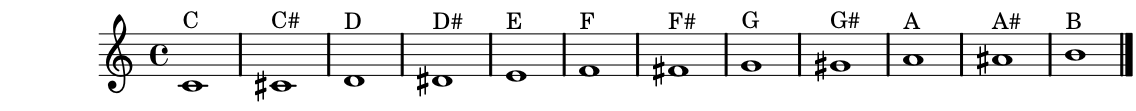
\includegraphics[angle=0, width=1\textwidth]{Cromatica.png}
\caption{\label{Cromatica}Escala Cromática.}
\end{figure}
Ahora bien, tómese cono ejemplo a la nota G. La nota que está un semitono arriba de ella es G$\sharp$; esta nota a su vez un semitono debajo de A, y de este modo, se le puede denotar también como A$\flat$. La propiedad de las notas de poseer múltiples nombres en la afinación equitemperada se llama \textbf{equivalencia enarmónica}\index{enarmónica, equivalencia}.

Como todos los múltiplos de una cierta frecuencia se representan con la misma letra, es conveniente representar a este conjunto de doce notas por medio de los enteros módulo 12, $\mathbb{Z}_{12}$. Una asignación posible es la que se puede ver en la figura \ref{Asignacion}, pero ésta no es rígida, ya que a cualquier nota (no sólo C) se le pudo haber asignado el $0$.

\begin{figure}[h]
\centering
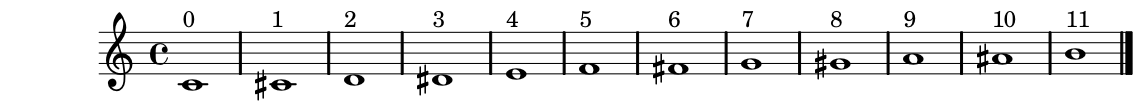
\includegraphics[angle=0, width=1\textwidth]{Asignacion.png}
\caption{\label{Asignacion}Correspondencia posible entre la escala cromática y $\mathbb{Z}_{12}$.}
\end{figure}

\section{El \emph{Gradus ad Parnassum} de Fux}\index{Gradus ad Parnassum}

\subsection{Intervalos y Consonancias}

De acuerdo a Johann Joseph Fux en su libro \emph{Gradus ad Parnassum}, el unísono, la tercera, la quinta, la sexta y la octava y los intervalos hechos de éstas son consonancias\index{consonancias}. Algunas de éstas son perfectas\index{consonancias!perfectas} y otras imperfectas\index{consonancias!imperfectas}. El unísono, la quinta y la octava son perfectas. La sexta y la tercera son imperfectas. Los intervalos restantes, como la segunda, la cuarta, la quinta disminuida, el tritono, la séptima y los intervalos hechos de éstas y la octava, son disonancias\index{disonancias}.

A manera de simplificar la definición de los diferentes intervalos, se pueden considerar como elementos en $\mathbb{Z}_{12}$. En el cuadro~\ref{CuadroIntervalos} puede verse esta asignación. 

\begin{table}[h]
\centering
\begin{tabular}{| c | c | l |}
\hline
$p$ & $0$ & unísono \\
$d$ & $1$ & segunda menor (o unísono aumentado)\\ 
$d$ & $2$ & segunda mayor \\
$i$ & $3$ & tercera menor (o segunda aumentada) \\
$i$ & $4$ & tercera mayor\\
$d$ & $5$ & cuarta justa\\
$d$ & $6$ & quinta disminuida (o cuarta aumentada o tritono) \\
$p$ & $7$ & quinta justa \\
$i$ & $8$ & sexta menor (o quinta aumentada) \\
$i$ & $9$ & sexta mayor \\
$d$ & $10$ & séptima menor (o sexta aumentada) \\
$d$ & $11$ & séptima mayor \\
$p$ & $12$ & octava justa \\
\hline
\end{tabular}
\caption{\label{CuadroIntervalos}Asignación entre los distintos tipos de intervalos y $\mathbb{Z}_{12}$.} 
\end{table}

La letra \emph{p} a la izquierda de un tono significa que es una consonancia perfecta, la \emph{i} que es una consonancia imperfecta y la \emph{d} que es una disonancia.

\subsection{Tipos de Movimiento}

Según Fux, el movimiento en música denota la distancia que se cubre al pasar de un intervalo a otro en una de dos direcciones, hacia arriba o hacia abajo. El movimiento directo\index{movimiento!directo} resulta de que dos o más partes asciendan o desciendan en la misma dirección, ya sea por intervalo o por salto (figura \ref{Directo}).
\begin{figure}[h]
\centering

\includegraphics[angle=0, width=1\textwidth]{Directo.png}
\caption{\label{Directo} Movimiento Directo.}
\end{figure}

El movimiento contrario\index{movimiento!contrario} tiene lugar cuando una parte asciende por intervalo o salto y la otra desciende o viceversa (figura \ref{Contrario}).
\begin{figure}[h]
\centering 

\includegraphics[angle=0, width=1\textwidth]{Contrario.png} 
\caption{\label{Contrario}Movimiento Contrario.}
\end{figure}

El movimiento oblicuo\index{movimiento!oblicuo} sucede cuando una parte se mueve por intervalo o salto mientras la otra permanece en el mismo lugar (figura \ref{Oblicuo}).
\begin{figure}[h] 
\centering 

\includegraphics[angle=0, width=1\textwidth]{Oblicuo.png} 
\caption{\label{Oblicuo}Movimiento Oblicuo.}
\end{figure}

\subsection{Las Cuatro Reglas Fundamentales}

Después de haber definido los tipos de movimiento, Fux define cuatro reglas fundamentales para usarlas en la práctica:

\begin{enumerate}
\item De una consonancia perfecta a otra perfecta, se debe proceder en movimiento contrario 	u oblicuo.
\item De una consonancia perfecta a una imperfecta, se puede proceder en cualesquiera de 		los tres tipos de movimiento.
\item De una consonancia imperfecta a una imperfecta se debe proceder en en movimiento 		contrario u oblicuo
\item De una consonancia imperfecta a una imperfecta, se debe proceder en cualesquiera de 	los tres movimientos.
\end{enumerate}

Usando respectivamente las letras $p$ e $i$ para las consonancias perfecta e imperfecta, y las letras $d$, $c$ y $o$ para los movimientos directo, contrario y oblicuo, estas cuatro reglas se pueden ver gráficamente en la figura \ref{Reglas}.

\selectlanguage{english}

\begin{figure}[h]
\centering 
\begin{tikzpicture}[shorten >=3pt,node distance=4cm,auto,every node/.style={font=\small\itshape}] 

	\node[state] (p)	                  {$p$}; 
	\node[state] (i) [right of=p] {$i$}; 


	\path[->] (p) edge [bend left]       node {d c o} (i)
                               edge [loop above]  node {c o}    (p)
                          (i) edge [bend left]	node {c o} (p)
                               edge [loop above]  node {d c o} (i);
\end{tikzpicture}
\selectlanguage{spanish}
\caption{\label{Reglas}Grafo de las cuatro reglas fundamentales.}
\end{figure}  

\selectlanguage{spanish}	

Es fácil ver entonces por qué Martini reduce las cuatro reglas a una sola: no está permitido el movimiento directo hacia una consonancia perfecta.

\subsection{Contrapunto Nota contra Nota}\label{CNCN}\index{contrapunto!nota contra nota}

Para Fux, el contrapunto\index{contrapunto} se entiende como la composición musical (polifónica) escrita estrictamente de acuerdo a reglas específicas. El contrapunto llamado indistintamente de la primera especie\index{contrapunto!de la primera especie}, nota contra nota\index{contrapunto!nota contra nota} o simple\index{contrapunto!simple}\footnote{ Es importante hacer notar que en esta tesis sólo trabajaremos con este tipo de contrapunto.}, es la composición más sencilla de dos o más voces con notas de la misma duración, formada solamente de consonancias. La duración de las notas es irrelevante, excepto que debe ser la misma para todas. Se toma como base para esto una melodía dada o cantus firmus\index{cantus firmus}.

Las consonancias\index{consonancias} se pueden usar de manera irrestricta, salvo sus diferencias de uso correspondientes a los diferentes tipo de movimiento y la regla de que se deben usar más consonancias imperfectas que perfectas. La excepción ocurre al principio y al final, ya que ambos deben estar formados de consonancias. El principio deberá expresar perfección y el final, relajamiento. Esto se debe a que las consonancias imperfectas carecen específicamente de perfección y no pueden expresar relajamiento. Finalmente, en el penúltimo compás, debe haber una sexta mayor si el cantus firmus se encuentra en la parte inferior; y una tercera mayor si se encuentra en la parte superior. 

En la figura \ref{Contrapunto} se muestra un ejemplo que se analiza abajo de la misma.

\begin{figure}[h] 
\centering 
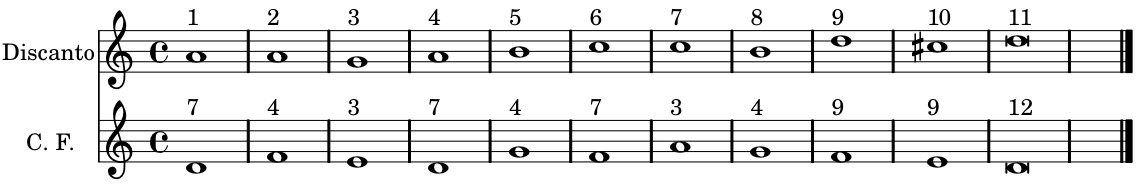
\includegraphics[angle=0, width=1\textwidth]{Contrapunto.png} 
\caption{\label{Contrapunto}Cantus Firmus (C. F.) y Discanto.}
\end{figure}

Para explicar el ejemplo, se toma a la nota de C como el $0$, a la de C sostenido como $1$, a la de D como $2$ y así sucesivamente.

\begin{description}
\item[1 (Primer compás).] El cantus firmus inicia con D ($2$), y de acuerdo a las reglas de Fux, se debe empezar con una consonancia perfecta, por lo que se elige la quinta justa: A ($2+7=9$).
\item[1--2] Si se escoge una consonancia perfecta, el movimiento sólo podrá ser contrario u oblicuo, pero si se elige una consonancia imperfecta, el movimiento puedes ser cualquiera de los tres. En este caso se escoge la tercera mayor de F ($5$), que es una consonancia imperfecta, obteniéndose A ($5+4=9$) a través de un movimiento oblicuo. 
\item[2--3] De una tercera mayor ($4$) a una tercera menor ($3$), o de una consonancia imperfecta a una consonancia imperfecta, se escoge el movimiento directo, aunque se pudo haber escogido cualesquiera de los otros dos. 
\item[3--4] De una tercera menor ($4$), una consonancia imperfecta, a una quinta justa ($7$), una consonancia perfecta, el movimiento es contrario. 
\item[4--5] De una consonancia perfecta ($7$) a una imperfecta ($4$), se usa uno de los tres tipos de movimiento permitido por las reglas: directo. 
\item[5--6] De una consonancia imperfecta ($4$) a una perfecta ($7$), movimiento contrario.
\item[6--7] Movimiento oblicuo, donde de hecho es imposible cometer un error.
\item[7--8] De una consonancia imperfecta ($3$) a una imperfecta ($4$), movimiento directo. 	
\item[8--9] De una consonancia imperfecta ($4$) a una imperfecta ($8$), se es libre de escoger cualquier tipo de movimiento. 
\item[9--10] Sucede lo mismo que en el anterior. 
\item[10 (Penúltimo).] Ya que el décimo compás es el penúltimo y el cantus firmus en éste se encuentra en la voz inferior, se escoge una sexta mayor ($9$) de acuerdo a la regla. 
\item[10--11] Finalmente, de una consonancia imperfecta ($9$) a una perfecta ($12$), el movimiento se escoge contrario. 
\item[11 (Último compás).] La conclusión, el décimo primer par de notas, es una consonancia perfecta ($12$).  
\end{description}

\section{Contrapunto Doble, Triple y Cuádruple}\label{Doble}

El \textbf{contrapunto doble}\index{contrapunto!doble} es un modo de composición que, sin violar las reglas del contrapunto estricto, le da a la melodía un contrapunto que se puede usar como la parte inferior o la parte superior  de dicha melodía. Esta técnica se conocía en la polifonía del siglo XVI, pero tuvo gran importancia por primera vez, en la fuga instrumental del siglo XVIII. Estudiaremos este tipo de contrapunto porque pone de manifiesto el papel de las transformaciones afines en la música, y porque son parte fundamental del modelo de contrapunto que desarrollaremos en el capítulo siguiente. 

El \textbf{contrapunto doble en la octava}\index{contrapunto!doble en la octava} es el más usado; en éste, la voz superior se \textbf{transporta} una octava abajo, o la inferior una octava arriba. Al hacer esta inversión, es bien sabido que el unísono se convierte en octava, la segunda en séptima y así sucesivamente. El contrapunto doble en la octava puede ser visto también como el ejercicio de encontrar el inverso aditivo (módulo 12) de cada nota del cantus firmus y luego transportarla 0 semitonos. Viéndolo así se puede usar la notación $D_{oct}(x)=e^0 \circ (-1)$. Es decir, $D(x)=e^n \circ (-1)$ significa que hay que obtener el inverso de la nota $x$ del cantus firmus y $e^n$ que hay que transportarla la nota obtenida $n$ semitonos. Ver el cuadro~\ref{CuadroDoble8}. En el siguiente capítulo, en la sección~\ref{Intervalos} está representación tendrá sentido. 

\begin{table}[h]
\centering
\begin{tabular}{|c c c c c c c c c c | }
\hline
C. F. & $x$ & $0$ & $2$ & $4$ & $5$ & $7$ & $8$ & $10$ & $0$\\
Discanto & $D_{oct}(x)$ & $0$ & $10$ & $8$ & $7$ & $5$ & $4$ & $2$ & $0$\\ 
\hline
\end{tabular}
\caption{\label{CuadroDoble8}Contrapunto doble en la octava.}
\end{table}

Como puede verse, todos los intervalos conservan su carácter de consonancias o disonancias según sea el caso, a excepción de la cuarta, la cual se convierte en quinta y viceversa. El ejercicio  del contrapunto doble en la octava no presenta problema alguno, y no contradice a las reglas usuales de las combinaciones de intervalos salvo una excepción: que la quinta se vea también como disonancia. Si se desea que dos voces no se crucen, el intervalo que existe entre ellas no deberá exceder una octava. Un ejemplo del contrapunto doble en la octava se puede ver en la figura \ref{Doble8}.

\begin{figure}[h]
\centering
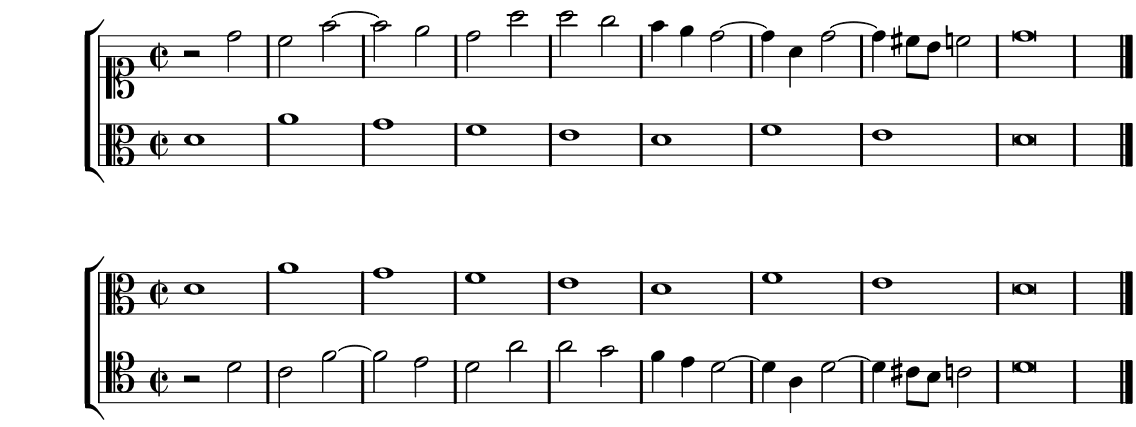
\includegraphics[angle=0, width=1\textwidth]{Doble8.png}
\caption{\label{Doble8}Ejemplo de contrapunto doble en la octava.}
\end{figure}

Si en el contrapunto doble en la octava se prohibe todo movimiento directo y todas las disonancias suspendidas, se le puede agregar a cada parte, arriba, una parte paralela en la tercera o décima, y de este modo se obtiene una composición a cuatro voces (figura~\ref{Cuadruple}).

\begin{figure}[h]
\centering
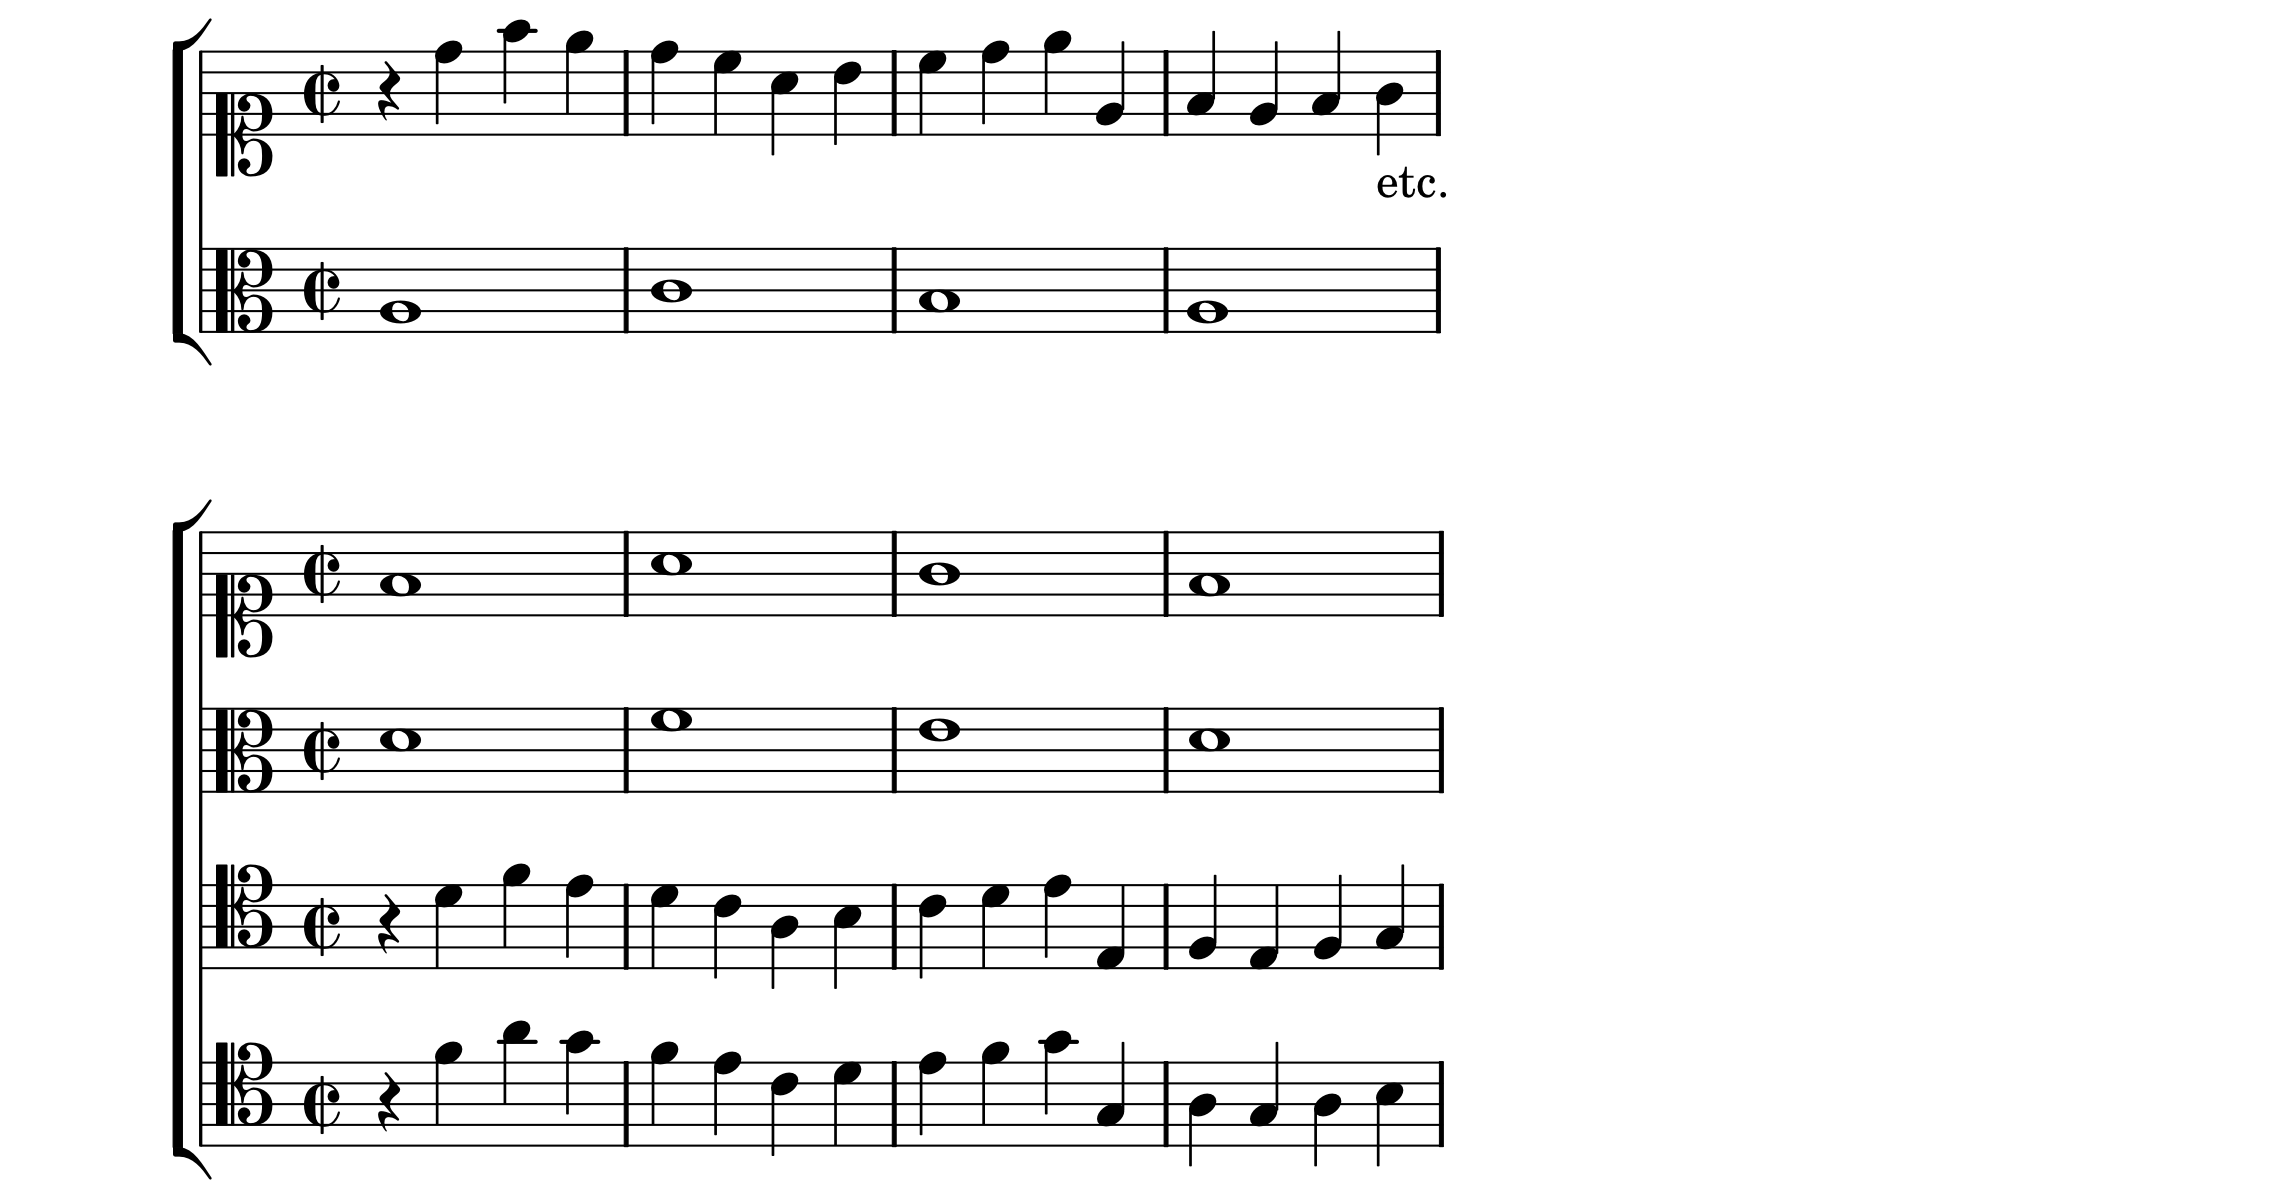
\includegraphics[angle=0, width=1\textwidth]{Cuadruple.png}
\caption{\label{Cuadruple}Ejemplo de contrapunto cuádruple.}
\end{figure}

Después del contrapunto en la octava, el contrapunto en la décima\index{contrapunto!doble en la décima} y en la doceava\index{contrapunto!doble en la doceava} se encuentran entre las formas más comunes. La inversión en la décima, usando la misma notación del contrapunto doble en la octava, cambia los intervalos aplicando la siguiente función $D_{dec}(x)=e^4 \circ (-1)$, como se puede ver en el cuadro~\ref{CuadroCuadruple}.

\begin{table}[h]
\centering
\begin{tabular}{| c c c c c c c c c c c c|}
\hline
C. F. & $x$ & $0$ & $2$ & $4$ & $5$ & $7$ & $9$ & $11$ & $0$ & $2$ & $4$\\
Discanto & $D_{dec}(x)$ & $4$ & $2$ & $0$ & $11$ & $9$ & $7$ & $5$ & $4$ & $2$ & $0$\\ 
\hline
\end{tabular}
\caption{\label{CuadroCuadruple}Contrapunto cuádruple.} 
\end{table}

Por lo tanto, todas las consonancias conservan su carácter de consonancias, tal como las disonancias permanecen disonantes después de invertirlas. Pero las consonancias perfectas se vuelven imperfectas, y las imperfectas perfectas; las terceras y las sextas paralelas así como las progresiones en movimiento directo a terceras y sextas, son por lo tanto inservibles. En otras palabras, sólo los movimientos contrario y oblicuo son posibles en estos ejercicios. Las suspensiones disonantes no se pueden usar, porque las cuartas, séptimas y segundas, manejadas correctamente, deben de terminar como en el caso de la inversión: séptimas en octavas, cuartas en quintas y novenas en octavas (figura \ref{Doble10}).

\begin{figure}[h]
\centering
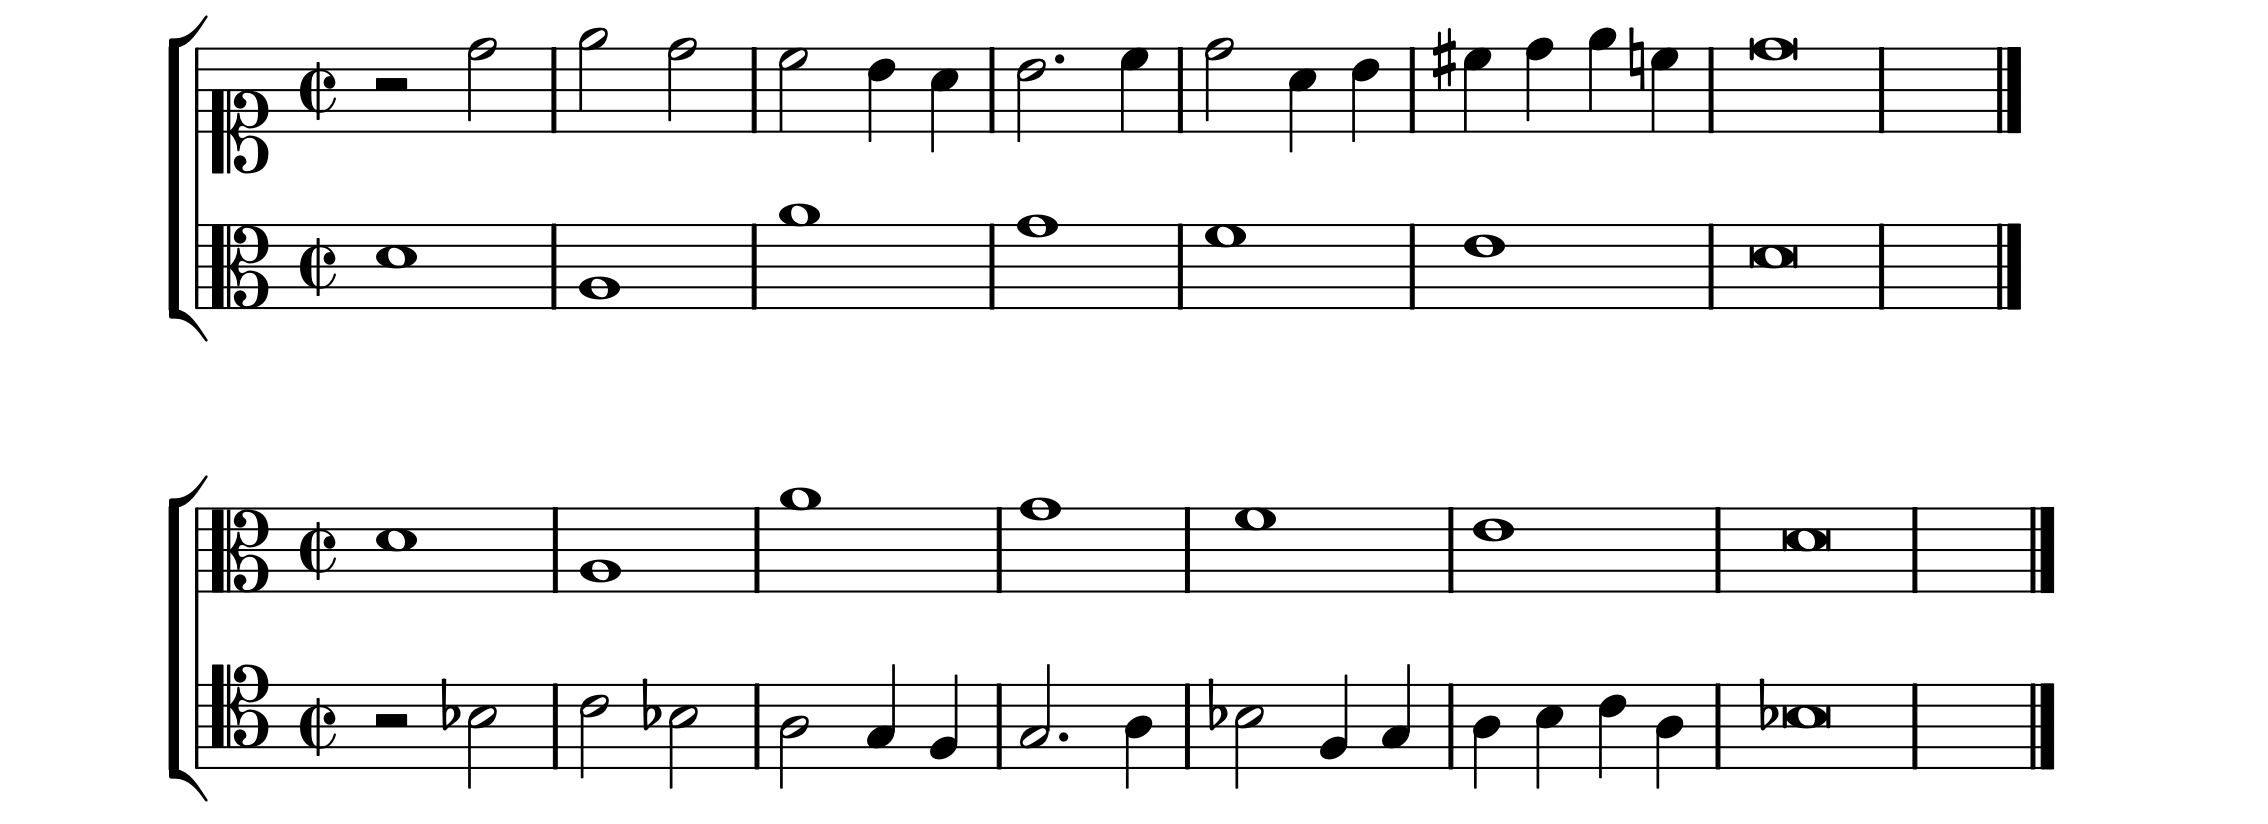
\includegraphics[angle=0, width=1\textwidth]{Doble10.png}
\caption{\label{Doble10}Ejemplo de contrapunto doble en la décima.}
\end{figure}
  
  En este caso, se puede incrementar en uno el número de partes si se añade ya sea una parte paralela en la décima abajo a la voz superior, o una en la décima arriba a la voz inferior, como se puede ver en la figura \ref{Triple}.

\begin{figure}[h]
\centering
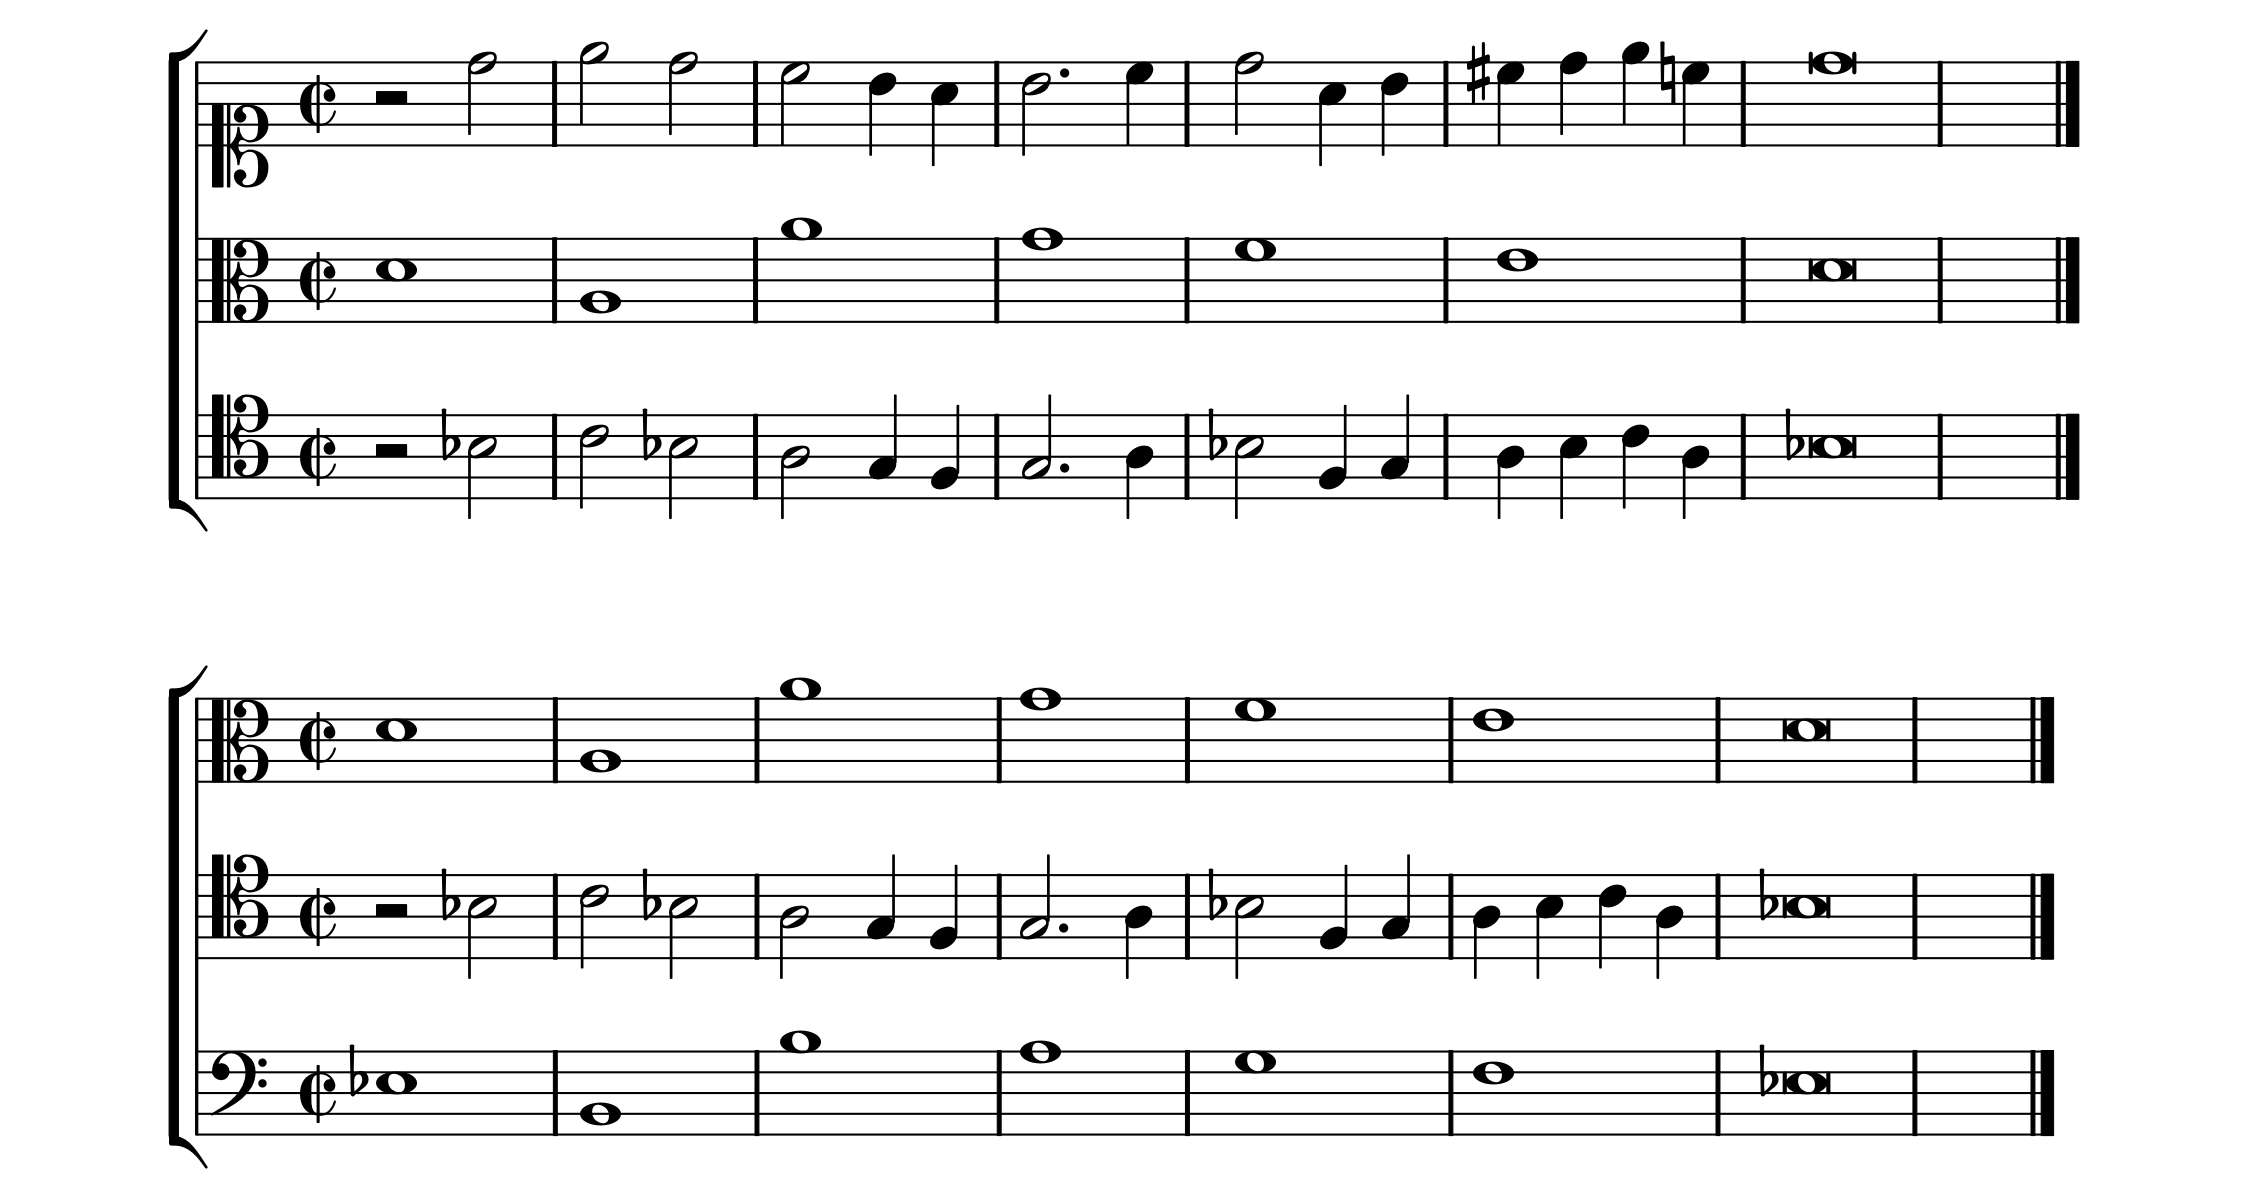
\includegraphics[angle=0, width=1\textwidth]{Triple.png}
\caption{\label{Triple}Ejemplo de contrapunto triple.}
\end{figure}

En la inversión en la doceava los intervalos se alteran de la siguiente manera, que puede verse también como la aplicación de la función $D_{doc}(x)=e^7 \circ (-1)$. Ver el cuadro~\ref{CuadroDoble12}.

\begin{table}[h]
\centering
\begin{tabular}{|c c c c c c c c c c c c c c|}
\hline
C. F. & $x$ & $0$ & $2$ & $4$ & $5$ & $7$ & $9$ & $10$ & $0$ & $2$ & $3$ & $5$ & $7$\\
Discanto & $D_{doc}(x)$ & $7$ & $5$ & $3$ & $2$ & $0$ & $10$ & $9$ & $7$ & $5$ & $4$ & $2$ & $0$\\ 
\hline
\end{tabular}
\caption{\label{CuadroDoble12}Contrapunto doble en la doceava.} 
\end{table}

El punto clave que hay que observar aquí es que la sexta, después de invertirla, se convierte en séptima, y consecuentemente, se debe tratar como disonancia. Además, si se prohiben las suspensiones y progresiones en movimiento directo, se puede hacer el ejercicio a tres o cuatro partes añadiendo voces paralelas en terceras o décimas sobre la voz inferior o debajo de la superior:

El contrapunto en más de dos partes es conocido como  \textbf{contrapunto triple}\index{contrapunto!triple} si tiene tres partes,  \textbf{cuádruple}\index{contrapunto!cuádruple} si tiene cuatro partes, y así sucesivamente. Es necesario que cada voz se mueva de acuerdo a las reglas de Fux. En este tipo de contrapunto, cuando está en la octava, las quintas deben tratarse como disonancias, sin importar las voces en las que ocurren. Debe hacerse notar que las cuartas no se pueden cubrir poniéndoles consonancias por debajo, como en el contrapunto simple.   

\chapter{El Modelo Matemático del Contrapunto}

\section{La Creación del Modelo}

\subsection{Historicidad y Sistema}

La música hace entrever, a muchos niveles de su realidad, la interacción esencial entre la temporalidad y la lógica, algo que se hizo evidente en el capítulo anterior. En primer lugar, a nivel de la obra individual, se observa la aplicación de la lógica de la composición en el desarrollo de los acontecimientos sonoros. Este tipo de interacción se ha encontrado también en el curso del análisis creador y de la reconstrucción de la composición de la que emana. 

Hablando de forma más general, de la evolución de las obras de un compositor dado, y por lo tanto de las grandes corrientes históricas de la música, se desarrolla un despliegue de la lógica progresiva del pensamiento musical en las obras, que se sumergen en el eco mental del escucha. Ahora bien, este tipo de interacción es menos verdadero que el primero:  mientras que la lógica del pensamiento de la composición se observa claramente en la temporalidad de una partitura, la naturaleza o la lógica directriz de la evolución histórica nunca es clara.

Para comprender el problema, hay que distinguir de entrada la historicidad en el proceso de descubrir leyes. Por ejemplo, el conocimiento de la anatomía de los objetos sonoros, tal como lo proporciona la descomposición de Fourier, obedece a la historia, pero la ley no es una función de historicidad\index{historicidad}. En Física, el descubrimiento de la transformación de Lorentz no es un cambio de la ley de transformación de Galileo, sino el desarrollo de nuestro conocimiento. No es un tipo simple de historicidad del que se habla aquí, sino un cambio de las mismas leyes y de la dinámica de la composición debido a leyes globales, tales que sean responsables, en Física, del enfriamiento del universo después de la estabilización de las leyes de la Era de Planck\index{Planck, Era de}.   

En este capítulo vamos a discutir precisamente una ley global responsable del resultado fuxiano de las reglas de contrapunto como fueron establecidas desde su primera aparición en el siglo XIX.

La cuestión subyacente a tal enfoque es sin duda la de su necesidad. ¿La historia de la música está necesariamente en interacción con principios atemporales? ¿Qué puede uno aprender de tal relación si verdaderamente tuvo lugar?

La musicología\index{musicología} se estableció sobre todo como una ciencia historiográfica en el sentido estricto del término y por lo tanto, no pudo proporcionar una respuesta a esta pregunta. Tenemos la tendencia a contentarnos con describir la sucesión histórica de los acontecimientos más allá de este orden histórico banal. El musicólogo Karl Dalhaus está claramente en contra de esta reducción radical: ``Sólo la construcción sistemática abre la visión a los hechos de una historia, que parezca valer la pena de ser contada''\cite{Verite}.
 
 Ahora bien, ¿por qué se debería insistir en una lógica sin tomar en cuenta el tiempo de la historia de la música? Para empezar, el orden histórico exclusivo reduce la coherencia al factor temporal y eso destruye la lógica inherente en beneficio de la temporalidad pura. A su vez, al hacer esto se destruye toda posibilidad de comparar los hechos más allá de su tiempo. Pero la historiografía\index{historiografía} debe ser la de una identidad que perdure por todos los tiempos. En otras palabras, hablar de música supone un sistema que crea su identidad en su evolución histórica y, por supuesto, cultural. El curso del tiempo ofrece el soporte sintagmático del despliegue de un sistema atemporal, ya sea por la obra individual, o por el desarrollo global de la música. Por lo tanto, la necesidad de este sistema resulta de la necesidad de identidad de la propia música.
 
 El problema resultante es el de la construcción de esta identidad sistemática. Es una construcción y no un descubrimiento, así que la historia de las ideas será ésa que construyamos y no la que encontremos ya hecha. La sustancia de la cual este sistema estará compuesto es la de la Matemática. Es nuestro postulado fundamental, un postulado alimentado por el paralelo hecho con la Física, y por el hecho de que la Matemática\index{Matemática} es el único dominio de la actividad humana mental que reúne precisión y abstracción.
 
Nuestro proceso de identificación parte del análisis creativo de los hechos que son entonces repensados en las fórmulas matemáticas, y además, tanteando a lo largo de la epidermis del comportamiento dentro de un dominio del saber que no es inductivo ni deductivo, sino un descubrimiento de las dimensiones según las cuales una problemática puede estar definida.

\subsection{Del Análisis Creador a la Creación de Modelos}
 
 La cuestión aquí es saber si la dinámica de la composición dentro de un modelo analítico dado, puede responder a las necesidades de la creación de las leyes de la música. Porque si el compositor fuera un simple productor industrial, no existiría ningún problema: se tendría una máquina de música.
 
 Para abordar la pregunta de la razón del funcionamiento de un sistema, hay que ponerlo en duda, es decir, explorar sus límites. Para comprender, hay que recorrer el proceso dialéctico de la doble negación: por qué el universo es tal como es, y no uno de tantos otros posibles dentro del universo múltiple, actual o potencial. En el momento en que lo hayamos caracterizado, será posible juzgar su naturaleza particular. 
 
 Para la composición musical, esta transgresión es particularmente importante, ya que la razón de la belleza no ha sido, a pesar de los esfuerzos  y las afirmaciones de los más grandes compositores, descubierta aún: se puede decir que ciertas construcciones son bellas, pero no se puede decir por qué. Resta todavía explorar la lógica de esta verdad. No se trata de un delirio de destrucción que no cesa de orillar a los creadores de la música a sus revoluciones incesantes. Se trata más bien del eje de la \emph{revolutio musicarum}\index{revolutio musicarum} que ellos se esfuerzan en hacer girar para comprender la orientación esencial. 
 
 Es este eje, no cabe duda, el que crea la identidad de la música, el invariante que estabiliza la evolución de la música en el curso de la historia. Si la verdad de la belleza no tuviera este recurso, el término \emph{belleza}\index{belleza} sería degradado a ornamentación efímera, de la que la cultura tendría el valor de un pasatiempo. La creación de este modelo juega entonces el papel de una investigación fundamental en vista de orientar el eje de rotación musical. Evidentemente, la hipótesis subyacente es que tal orientación axial existe, a partir de ahora o después de llevar a cabo un desarrollo más profundo.
 
\subsection{Pensar Hoy la Música del Futuro}
 
 Para pensar hoy la música del futuro, hay que saber cómo hacer girar el eje de rotación. Hay que reflexionar sobre los medios y técnicas aptos para concebir y proyectar en la imaginación las estructuras futuras de lo sonoro. 
 
 Al proseguir con la metáfora del eje de rotación, su rotación hacia el futuro debe hacerse identificando la posición actual del pensamiento musical como ángulo específico de rotación, y a continuación, poniendo en marcha una dinámica de cambio de posición, de cambio de ángulo.
 
 Esta estrategia no es otra que la del reconocimiento del estado de las cosas como un caso particular de un hecho general. La elección histórica representaba entonces una perspectiva particular del hecho general, un punto de vista bajo un ángulo que deberíamos de cambiar para reconocer una perspectiva nueva. La creación en juego sería entonces de ese hecho general y no la elección de un nuevo ángulo, que no constituía más que un paso arbitrario en la exploración genérica.
 
 La construcción del hecho general que vamos a presentar a continuación se refiere al campo del contrapunto clásico de Fux. Es en esta teoría de composición en la que nos vamos a adentrar dentro de un marco conceptual general de potencial ``revolucionario''. Para comprender este proyecto, sería didáctico reconsiderar el enfoque clásico en comparación con la revolución en el núcleo de la tradición contrapuntística: la dicotomía de las cualidades interválicas en consonancias y disonancias. Es la invención de la técnica dodecafónica\index{dodecafónica, técnica} por Arnold Schoenberg\index{Schoenberg, Arnold}, de la que el primer vestigio se encuentra plasmado en el \emph{Vals n. 5} op. 23 para piano. Según Theodor Wiesengrund Adorno\index{Adorno, Theodor Wiesengrund}, la emancipación schoenberguiana de las disonancias representa la respuesta progresista a la tradición tonal. Y Schoenberg estuvo orgulloso de ella, al punto de estar seguro de que esta invención aseguraría la primacía de la música alemana por un siglo. 
 
 La construcción dodecafónica instala una serie y sus transformaciones compuestas de retrogradación\index{retrogradación}, inversión\index{inversión} e inversión retrógrada\index{inversión!retrógrada}\footnote{En la retrogradación, la serie original se toma empezando por el final; en la inversión, todos los intervalos se imitan pero en movimiento contrario; la retrogradación de la inversión es la combinación de las dos primeras.}, sin calificar o descalificar los aspectos interválicos que de éstas se deducen. Estos aspectos son interrumpidos por criterios opuestos a la armonía\index{armonía!tonal} tonal. Esta estrategia es entonces una aniquilación del pensamiento tonal basado en la dicotomía\index{dicotomía} consonancias contra disonancias. No se podrá entonces hablar aquí de un hecho general en el que la armonía tonal fuere una perspectiva particular, y entonces el dodecafonismo fuere el resultado de una ``revolución rotativa''. Es, más bien, una ruptura radical, una negación del concepto mismo de las cualidades armónicas.
 
 Nuestro plan difiere entones cualitativamente de la invención schoenberguiana; nosotros procedemos utilizando la tradición dialéctica de la sustitución de una tesis por su doble negación y no usando la tradición de la ruptura total. Para hacer eso, nuestra estrategia consiste primeramente en la modelación del contrapunto fuxiano en una conceptualización matemática de modo que las reglas clásicas se deduzcan. A continuación, se coloca el contexto clásico en un marco matemático que se deriva del marco fuxiano, es decir, que se reconoce que los axiomas y teoremas que definen el modelo matemático de la teoría fuxiana se generalizan sin dificultad y crean entonces los modelos alternativos, mundos contrapuntísticos ``exóticos'', que proponen perspectivas variadas del modelo genérico, al englobar el modelo específico del marco fuxiano.
 
 La negación consiste entonces en la invención de un hecho general, de este eje que permanece fijo en el curso de la Historia, y entonces los ángulos específicos apuntan a las instancias temporales de la historia de la música. La negación y la doble negación están relacionadas por la dualidad de la atemporalidad matemática frente a la temporalidad histórica. La fórmula matemática da lugar a los hechos de la música para el desarrollo de un acto que sobresale con el paso del tiempo.
 
\section[Los Intervalos de Contrapunto]{Los Intervalos de Contrapunto son \\*Tangentes Geométricos}
 
\subsection{Conceptos Algebraicos}
 
 Para el modelo de contrapunto, vamos a trabajar con el conjunto $\mathbb{Z}_{12}$ que se introdujo en la sección \ref{Fundamentos}: en la teoría clásica de contrapunto de Fux podemos no considerar más que los intervalos menores a la octava. A continuación justificaremos esta hipótesis, no sin antes afirmar que vamos a apoyarnos en ella con el fin de construir un modelo estrictamente modular de contrapunto. A partir de este momento, los conceptos matemáticos necesarios para tal fin se irán definiendo a medida que los vayamos necesitando.
 
\begin{Def} \label{Grupo} 
 Un \textbf{grupo}\index{grupo} es una pareja $(G,\cdot)$ donde $G$ es un conjunto no vacío, $\cdot:G \times G \to G$ es una operación binaria $(x,y) \mapsto \cdot (x,y)=x \cdot y = xy$, tal que:
 \begin{enumerate}
  \item $(xy)z=x(yz); x,y,z \in G$
  \item existe un elemento $e \in G$ tal que $ey=ye=y$, para toda $y \in G$  
  \item para cada $y \in G$ existe un elemento, denotado $y^{-1}$, tal que $(y^{-1})y=y(y^{-1})=e$.
 \end{enumerate}
\end{Def}
 
\begin{Def}
 Un \textbf{subgrupo}\index{subgrupo} es un subconjunto no vacío de un grupo el cual en sí mismo es un grupo. Al subgrupo del grupo multiplicativo $(G,\cdot)$, $\{x^n | n \in \mathbb{Z}\}$ denotado por $(x)$, se le conoce como  \textbf{subgrupo cíclico}\index{subgrupo!cíclico} de $G$ generado por $x$. Si existe un número natural $n$ y es el más pequeño tal que $x^n=e$, se dice que $(x)$ es un \textbf{grupo cíclico de orden}\index{grupo!cíclico de orden $n$} $n$. Si no existe, a $(x)$ se le llama \textbf{grupo cíclico infinito}\index{grupo!cíclico infinito}.
\end{Def}
   
\begin{Def}
 Sean $(G,\cdot)$ y $(G',\ast)$ dos grupos. Un \textbf{homomorfismo de grupos}\index{homomorfismo!de grupos} es una función $f:G \to G'$ tal que $f(u \cdot v)=f(u) \ast f(v)$. Si además $f$ tiene inversa, a $f$ se le conoce como \textbf{isomorfismo}\index{isomorfismo!de grupos} y se dice que $G$ y $G'$ son \textbf{isomorfos}\index{isomorfos}.
\end{Def}

Veamos ahora los siguientes teoremas, también necesarios para la justificación.

\begin{Teo} 
Sea $(G,\cdot)$ un grupo cíclico infinito\index{grupo!cíclico infinito}. Entonces, si $x$ es un elemento fijo de $G$, la función $h:\mathbb{Z}\to G:n\mapsto x^n$ es un isomorfismo de grupos\index{isomorfismo de grupos}.
\end{Teo}

\begin{Teo} 
Sea $(x)$ un grupo cíclico generado por $x$ y $h:(x)\to H$ un homomorfismo de grupos\index{homomorfismo!de grupos}. Entonces $h((x))$ es un subgrupo cíclico\index{subgrupo!cíclico} de $H$.
\end{Teo}

Por último, una definición relevante:

\begin{Def} 
 Sea $(G,\cdot)$ un grupo abeliano\index{grupo!abeliano}, $(H,\cdot)$ un subgrupo de $G$ y $x \in G$. Al conjunto $\{xy | y \in H\}$ que denotaremos por $xH=Hx$, se le denomina \textbf{clase lateral}\index{clase lateral} de $H$ en $G$. Si formamos el conjunto de todas las clases laterales de $H$ en $G$, denotado por $G/H$ y definimos la operación binaria $\cdot:G/H \times G/H \to G/H:(xH,yH) \mapsto xyH$ se obtiene un grupo. A $(G/H,\cdot)$ se le conoce como el \textbf{grupo cociente}\index{grupo!cociente} de $G$ módulo $H$.
\end{Def}

 Estamos en condiciones de justificar la hipótesis de que podemos no considerar más que los intervalos menores a la octava. Para empezar, recalcamos que $(x)$ es un subgrupo de los números reales sin incluir al cero. Pues bien, se sabe que el cerebro humano percibe dos tonos como esencialmente idénticos cuando sus frecuencias guardan una razón igual a $2^r$, con $r \in \mathbb{Z}$. Es decir, el cerebro ``identifica'' dos frecuencias $u, w \in (x)$, subgrupo de $(\mathbb{R}-\{0\},\cdot)$, cuando $w=v\cdot h$ para alguna $h \in (x^{12})$ y donde $x$ es el número real $x=\sqrt[12]{2}$. En efecto, $x^{12}=2$ y $w=v\cdot h=v\cdot(2)$ significa que $\frac{w}{v}=2^r$ para algún $r \in \mathbb{Z}$. Por otro lado, puesto que $h:\mathbb{Z} \to (x):n \mapsto x^n$ define un isomorfismo entre $\mathbb{Z}$ y $(x)$, resulta que para la percepción humana, los tonos esencialmente distintos son aquéllos del cociente $(x)/(x^{12})$ isomorfo a  $\mathbb{Z}/12\mathbb{Z}=\mathbb{Z}_{12}$, ya que puede demostrarse que $(x^{12})$ es isomorfo a $12 \mathbb{Z}$ bajo el isomorfismo $h$. 
 
 Ahora bien, el hecho de identificar a un elemento de $\mathbb{Z}$ por uno de $\mathbb{Z}_{12}$, es muy útil para definir el concepto de escala. Una \textbf{escala}\index{escala} $E$ es un subconjunto de $\mathbb{Z}$, al que vemos como tonos, tal que $e^{12}(E)=E+12=E$. Es decir, $x+12 \in E$ para todo $x \in E$. Un ejemplo conocido para nosotros es la escala cromática\index{escala!cromática}, donde $E=\mathbb{Z}_{12}$.
 
\subsection{El Toro de Terceras}\label{ToroTerceras}\index{toro de terceras}
  
 Lo cierto es que si para nuestro modelo de contrapunto intentáramos trabajar únicamente con las simetrías de inversión y transporte en $\mathbb{Z}_{12}$, representando geométricamente a este grupo cíclico de orden $12$\index{geometría!de $\mathbb{Z}_{12}$} por un círculo como en una carátula de reloj, eso no nos sería suficiente. Veamos por qué. En el contrapunto, las quintas $(7)$ y las cuartas $(5)$ tienen un papel central. Así que necesitaremos en particular simetrías\index{simetrías} de $\mathbb{Z}_{12}$ de la forma $m(x)=7x+b$ ó $m(x)=5x+b$, es decir, que tengan multiplicadores relacionados a las quintas y a las cuartas. Desafortunadamente, la representación circular de $\mathbb{Z}_{12}$ muestra una geometría transformada cuando se le multiplica por $5$ ó por $7$. Porque si las alturas $x_1, x_2$ se separan $x_1-x_2$, sus imágenes $m(x)=7x_1+b, m(x)=7x_2+b$, difieren por $7(x_1-x_2)$. Por ejemplo, si $x_1-x_2=1$  (un semitono), sus imágenes difieren por una quinta. 
 
 Este problema se puede eliminar a través de un procedimiento matemático muy clásico que se muestra, al mismo tiempo, como un método que tiene un alcance musical. 
  
\begin{Teo}
Si $G$ es un grupo abeliano, es decir, conmutativo, y finito, entonces es isomorfo al producto directo de grupos cíclicos finitos de orden $m_i$, donde $m_i|m_{i+1}$ para $1 \le i \le n-1$. 
\end{Teo}
 
 Por el resultado anterior sabemos que $\mathbb{Z}_{12}$ es un grupo isomorfo al producto cartesiano   $\mathbb{Z}_{3} \times \mathbb{Z}_{4}$.  El isomorfismo que empleamos en nuestro contexto es el siguiente:
 
\begin{description}
\centering
 \item $ \phi: \mathbb{Z}_{12} \to \mathbb{Z}_{3} \times \mathbb{Z}_{4}$
 \item $ \phi(z)=(z,-z)$,
\end{description}
 y el homomorfismo inverso:
\begin{description}
\centering
 \item $ \phi^{-1}: \mathbb{Z}_{3} \times \mathbb{Z}_{4} \to \mathbb{Z}_{12}$
 \item $ \phi^{-1}(u,v)=4u+3v$.
\end{description}

 Este isomorfismo es muy importante para la teoría de la música, ya que el número de la tercera mayor $4$ se manda al par $(1,0)$, mientras que la tercera menor $3$ se envía a la pareja $(0,1)$. Esto significa que el par $(u,v)$ representa un intervalo compuesto de $u$ terceras mayores y de $v$ terceras menores.
 
 Una representación geométrica del producto cartesiano $\mathbb{Z}_{3}$ $\times$ $\mathbb{Z}_{4}$, llamada \textbf{toro de terceras}\index{toro de terceras}, está dado por el toro discreto representado en la figura~\ref{Toro}. Los cuatro meridianos verticales representan los pasos de terceras menores, y los tres meridianos horizontales los pasos de terceras menores. La espiral representa el recorrido por semitonos.
 
\begin{figure}[h]
\centering
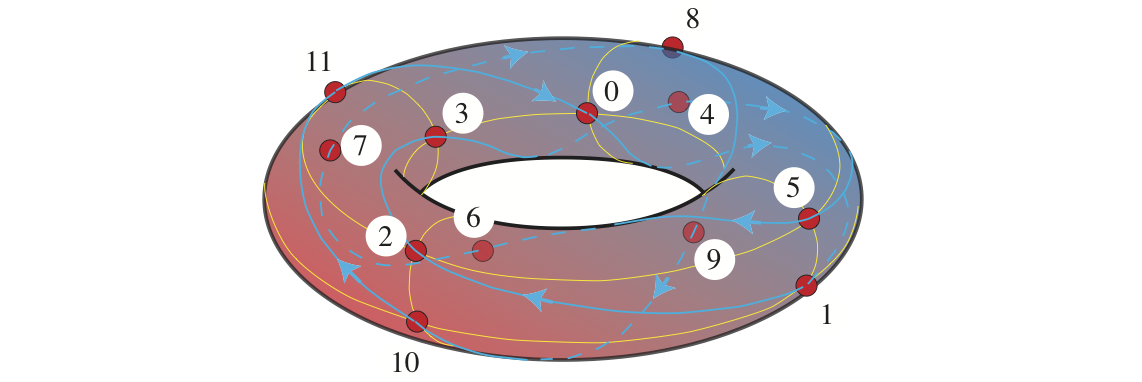
\includegraphics[angle=0, width=1\textwidth]{ToroColor.png}
\caption{\label{Toro}El toro de terceras.}
\end{figure}
 
 Ahora bien, en el toro de terceras se tiene una métrica canónica\index{métrica canónica}, la distancia $d(x,y)$ entre dos elementos $x,y \in \mathbb{Z}_{3} \times \mathbb{Z}_{4}$ que se define como el número mínimo de terceras menores o mayores necesarias para llegar a $y$ partiendo de $x$ (o viceversa); es el número mínimo de pasos ``elementales'' sobre los meridianos del toro para unir a $y$ partiendo de $x$. Por ejemplo, se tiene que $d(4,5)=2$ ó $d(3,0)=1$. Con esta métrica, se puede demostrar que toda simetría\index{simetría} $m(x)=ax+b$ con $a=1,5,7,11$ y no sólo para las traslaciones e inversiones, se conserva la distancia $d(m(x),m(y))=(x,y)$. Por ejemplo, la simetría $m(x)=5x$ se interpreta como la reflexión sobre el plano ecuatorial, que evidentemente conserva las distancias. Esto quiere decir que la geometría del toro de terceras\index{geometría!del toro de terceras} permite interpretar las simetrías como isometrías, hecho que no aparece en la geometría\index{geometría!de $\mathbb{Z}_{12}$} de la representación circular de $\mathbb{Z}_{12}$. 

\subsection{El Espacio de Tangentes}
  
  El contrapunto se construye sobre el concepto de intervalo que se extiende del  \emph{cantus firmus}\index{cantus firmus} $CF$ (melodía cerrada o primera) al \emph{discantus}\index{discanto} $D$ (discanto\index{discanto}). Este concepto define roles distintos del $CF$ con respecto a $D \subset \mathbb{Z}_{12}$. Se deberá proporcionar entonces una definición matemática de un intervalo de contrapunto\index{intervalo!de contrapunto} que considere esta asimetría. Lo haremos al escribir un intervalo como una expresión algebraica, de entrada puramente formal, $CF+\epsilon.(D-CF)$, donde la diferencia $D-CF$ mide la cantidad interválica entre el discanto y el cantus firmus. Esta aproximación se puede interpretar como una construcción geométrica de una tangente. La cantidad interválica $D-CF$ se interpreta como la tangente de longitud $D-CF$ con respecto al punto $CF$. Esta descripción puede parecer un poco artificial, pero se puede justificar por medio de dos argumentos: de entrada, el discanto es un tipo de ``variación'' del cantus firmus, una``vibración infinitesimal'',  entonces \emph{la tensión\index{tensión} con respecto al cantus firmus caracteriza la cualidad del contrapunto}. El segundo argumento es estrictamente matemático: en geometría algebraica, las tangentes están descritas por los \textbf{números duales}\index{números duales}, y estos números a su vez están descritos por las simetrías\index{simetrías} de tipo $c+\epsilon.d$.\footnote{Es importante mencionar también que los intervalos, vistos sin importar el cantus firmus $c$, son los que importan para el movimiento de las voces. Es decir, no importa cuál sea el``tono base'' de una quinta, sino el hecho de que sea una quinta.} 
  
  Antes de conocer a los números duales, es necesario definir algunos conceptos.
  
\begin{Def}
 Si en la definición \ref{Grupo} de grupo  se considera un conjunto $S$ con la operación binaria $\cdot$ que cumpla $(1)$, se dice que $(S,\cdot)$ es un \textbf{semigrupo}\index{semigrupo}.
\end{Def} 
  
 \begin{Def}
 Un \textbf{anillo}\index{anillo} es una terna $(R,+,\cdot)$ donde $R$ es un conjunto, $+$ y $\cdot$ son operaciones binarias tales que
 \begin{enumerate}
  \item $(R,+)$ es un grupo abeliano
  \item $(R, \cdot)$ es un semigrupo
  \item $u(v+w)=uv+uw$ y $(u+v)w=uw+vw$.
 \end{enumerate}  
\end{Def} 
  
 \begin{Def}
  Sea $R$ un anillo. Un $R$-\textbf{módulo}\index{módulo} es una terna $(R,M,\mu:R \times M \to M)$, donde $(M,+)$ es un grupo abeliano y $\mu$ es la multiplicación escalar, tal que:
 \begin{enumerate}
   \item para todo $m  \in M,1_R(m)=m$
   \item para todo $r,s  \in R$ y $m,n  \in M$, $(r+s)m=rm+sm, r(m+n)=rm+rn$ y $r(sm)=(rs)m$. 
  \end{enumerate}  
 \end{Def}
  
\begin{Def}
Si $k$ es un anillo conmutativo, entonces un anillo $R$ es una $k$-\textbf{álgebra}\index{álgebra} si a su vez es un $k$-módulo y los escalaras en $k$ conmutan con cualquier elemento:

\centering $ar(s)=(ar)s=r(as)$.  
\end{Def}
    
\begin{Def}
A la $\mathbb{Z}_{12}$-álgebra cuyos elementos son de la forma $c+\epsilon .d$, con $c,d \in \mathbb{Z}_{12}$, se le conoce como el álgebra de los \textbf{números duales}\index{números duales}. Se le denota $\mathbb{Z}_{12}[\epsilon]$.
\end{Def}  

Se tiene entonces que si $x_1+\epsilon.d_1,x_2+\epsilon.d_2 \in \mathbb{Z}_{12}[\epsilon]$:  
\begin{itemize}
\item[]$(x_1+\epsilon.d_1)+(x_2+\epsilon.d_2)=(x_1+x_2)+\epsilon.(d_1+d_2)$,
\item[]$(x_1+\epsilon.d_1)\cdot(x_2+\epsilon.d_2)=(x_1x_2)+\epsilon.(x_1d_2+x_2d_1)$,
\item[]y en particular, $\epsilon\cdot\epsilon=0$. 
\end{itemize} 

Por razones evidentes, este espacio es conocido como \textbf{espacio de tangentes}\index{tangentes, espacio de}; de aquí en adelante llamaremos a sus elementos \textbf{tangentes} o \textbf{intervalos de contrapunto}\index{contrapunto!intervalos de}. 

Es necesario reconocer aquí la aportación matemática en la conceptualización de las entidades musicales. No sólo se ha creado una representación precisa de la información interválica, sino también una estructura algebraica tomada de la geometría algebraica. Este acto es al mismo tiempo creativo y arriesgado: no sabemos cuáles serán las consecuencias para la teorización ulterior. Estas estructuras parecen potencialmente ricas, pero por el momento, no podemos afirmar si su utilización en el marco musical nos abrirá nuevos caminos.

\subsection{Orientación de Contrapunto}\label{Orientacion}

En la definición de un intervalo de contrapunto $c+\epsilon.d$, de algún modo el discanto pasa a segundo plano a favor del número interválico $d$, el coeficiente de $\epsilon$. Se tiene en efecto una ventaja para la teoría musical, ya que existen dos orientaciones de los intervalos: el \textbf{contrapunto barriente}\index{contrapunto!barriente} ($\Omega_+$), donde la voz del discanto está por encima del cantus firmus, 
y el \textbf{contrapunto colgante}\index{contrapunto!colgante} ($\Omega_-$), donde la voz del discanto se encuentra por debajo del cantus firmus. Estas dos orientaciones se pueden definir como funciones matemáticas:

\begin{description}
\centering
 \item $\Omega_\pm : \mathbb{Z}_{12}[\epsilon] \to\mathbb{Z}_{12} : c+\epsilon.d \mapsto c\pm d$, 
 \end{description}
 que asocian al intervalo $c+\epsilon.d$ el discanto $\Omega_\pm(c+\epsilon.d)=c\pm d$. A una orientación\index{orientación!fija} que esté fija, se le puede olvidar provisoriamente para describir las reglas de la sucesión de los intervalos de contrapunto $c_1+\epsilon.d_1,c_2+\epsilon.d_2$. Sin embargo, si debemos utilizar una sucesión acompañada de un cambio de orientación\index{orientación!cambio de}, por ejemplo de $\Omega_+$ a $\Omega_-$, entonces hay que encontrar un modo de fijar una orientación constante\index{orientación!constante}. La idea consiste en observar que esto se consigue haciendo lo siguiente:

\begin{description}
\centering 
 \item $\Omega_-(c+\epsilon.d)=\Omega_+((-1+\epsilon.$2$)\cdot(c+\epsilon.d))$, es decir, 
 \item $\Omega_-=\Omega_+\circ(-1+\epsilon.$2$)$, 
\end{description}
y se podrá entonces considerar el paso $c_1+\epsilon.d_1,(-1+\epsilon.$2$)\cdot(c_2+\epsilon.d_2)$ con la orientación constante $\Omega_+$, en lugar del paso $c_1+\epsilon.d_1,c_2+\epsilon.d_2$, que contenía un cambio de orientación. \emph{Por lo tanto, en nuestro modelo podemos fijar la orientación sin pérdida de generalidad.}

\section[La Autocomplementariedad Contrapuntística]{La Autocomplementariedad \\* Contrapuntística}

\subsection[La Autocomplementariedad para Tonos]{La Autocomplementariedad del Contrapunto \\* Clásico para Tonos} \label{AC}

Fijemos de una vez por todas la orientación $ \Omega_+$. El contrapunto clásico de Fux se centra alrededor de la situación principal del estilo ``nota contra nota''\index{contrapunto!nota contra nota}: se parte de una melodía $CF=c_1,c_2,\ldots c_n$ del cantus firmus y se debe asociar a cada nota $c_i$ de la melodía $CF$ un número interválico $d_i$ de tal modo que los intervalos $\alpha_i=c_i+\epsilon.d_i$ satisfagan un cierto número de condiciones que vamos a discutir a continuación. Los discantos asociados $DE_i=\Omega_+(\alpha_i)=c_i+d_i$ forman la melodía del discanto $DE=DE_1,DE_2,\ldots DE_n$. Esta melodía se toca simultáneamente con $CF$; se tendrá entonces un conjunto de parejas simultáneas $\{CF_i,DE_i\}$.
La primera regla para deducir $DE$ de $CF$ es que los números interválicos $d_i$ son todos \textbf{consonancias}\index{consonancias} contrapuntísticas, es decir, $d_i \in K=\{0,3,4,7,8,9\} \subset \mathbb{Z}_{12}$, cuyos respectivos nombres son \textbf{primera, tercera menor, tercera mayor, quinta, sexta menor} y \textbf{sexta mayor}. Este conjunto de seis números se completa por el conjunto de \textbf{disonancias}\index{disonancias} $D=\mathbb{Z}_{12}\setminus K=\{1,2,5,6,10,11\}$, denominados \textbf{segunda menor, segunda mayor, cuarta, tritono, séptima menor} y \textbf{séptima mayor}. 

\begin{Def}
Llamaremos \textbf{dicotomía} a la partición $(K|D)$ de $\mathbb{Z}_{12}$ en consonancias y disonancias, tal que los conjuntos $K$ y $D$ tienen la misma cardinalidad y $K \cup D=\mathbb{Z}_{12}$.
\end{Def}

Obsérvese que la \textbf{cuarta}\index{cuarta} no es una consonancia en esta teoría principal, un hecho que pone en duda las explicaciones acústicas de la dicotomía de las consonancias y las disonancias. El contrapunto no es una teoría acústica ni psicológica, sino ante todo, una teoría de composición. El musicólogo Karl Dalhaus \cite{Dalhaus} reconoce que la disonancia de la cuarta debe tener una justificación en términos de la lógica de la composición que aún no ha sido comprendida.

Si no es posible referirse a la base acústica para justificar la cualificación de la consonancia contrapuntística, hay que buscar otras explicaciones. Ahora bien, para hacer esto, trabajaremos primeramente únicamente con tonos para más tarde extender la teoría a los intervalos de contrapunto. Existen así dos posibilidades:
 
 \begin{enumerate}
\item Se busca encontrar atributos booleanos de las notas tales que su valor separe las consonancias de las disonancias . Es, de algún modo, lo que la acústica quería hacer, por ejemplo, por medio de las fórmulas de Leonard Euler\index{Euler, Leonard} (la función \emph{gradus suavitatis}\index{gradus suavitatis}) o las fórmulas de las pulsaciones entre sonidos parciales de Herman von Helmholtz\index{Helmholtz, Herman von}. De cierto modo, estas fórmulas no definen dicotomías sino más bien grados de consonancia. Hay entonces que introducir valores de separación artificiales para crear dicotomías. 
\item No se buscan atributos de los números individuales, sino de su conjunto. Ésta una posibilidad que no es equivalente a la primera, al utilizar la función característica de un subconjunto. Concretamente, podríamos buscar subconjuntos de $\mathbb{Z}_{12}$ que fueran cerrados bajo la multiplicación y que no tuvieran mas que seis elementos; como los números pares, por ejemplo.
\end{enumerate} 

La pareja que nos proporciona el conjunto $K$ de consonancias entre los subconjuntos $X$ de $\mathbb{Z}_{12}$ está definida por las propiedades siguientes:

\begin{enumerate}
\item Se pide que exista una sola simetría $m(x)=a.x+b$ que induzca una biyección $m:X \tilde{\to}$ $\mathbb{Z}_{12}\setminus X$; le llamaremos \textbf{simetría de autocomplementariedad de $X$}\index{simetría!de autocomplementariedad en $\mathbb{Z}_{12}$}, porque relaciona a un subconjunto $X$ de $\mathbb{Z}_{12}$ con su complemento $\mathbb{Z}_{12}\setminus X$. A tal dicotomía $(X|$ $\mathbb{Z}_{12}\setminus X)$ de $\mathbb{Z}_{12}$ se le llamará \textbf{dicotomía fuerte}\index{dicotomía!fuerte}.
\item Se pide que el conjunto $7.X$ sea cerrado bajo la multiplicación y que $7.X$ contenga al elemento neutro de la multiplicación $1$. A $7.X$ le podemos llamar \textbf{monoide\index{monoide!multiplicativo de quintas}\footnote{Si en la definición de grupo \ref{Grupo} se considera un conjunto $M$ con la operación binaria $\cdot$ que cumpla $(1)$ y $(2)$, se dice que $(M,\cdot)$ es un \textbf{monoide}.} multiplicativo de quintas} (múltiplos de $7$).
\end{enumerate} 

Un resultado sorprendente descubierto por T. Noll es que sólo el conjunto $K$ tiene esos dos atributos. Su función de autocomplementariedad es:
\begin{description}
\centering
\item $ m(x)=AC(x)=5x+2$. 
\end{description}

He aquí los valores:
\begin{description}
\centering
\item$AC(0)=2,AC(3)=5,AC(4)=10,AC(7)=1,AC(8)=6,AC(9)=11$.
\end{description}

Se verifica de manera inmediata que $AC \circ AC=Id$, la identidad sobre $\mathbb{Z}_{12}$, es decir, $AC$ es una \textbf{involución}\index{involución} en $\mathbb{Z}_{12}$ que intercambia $K$ y $D$. La unicidad de $AC$ se deriva de un argumento geométrico notable: si se relacionan los números consonantes dos a dos por medio de arcos, cada vez que su distancia es uno\footnote{La métrica utilizada aquí es la misma definida en la sección~\ref{ToroTerceras}.}, se obtiene la gráfica sobre $K$ mostrada en la figura \ref{Consonancias}. 

\selectlanguage{english}

\begin{figure}[h]
\centering 
\begin{tikzpicture}[shorten >=3pt,auto,node distance=3.5cm,every node/.style={font=\small\itshape}] 

	\node[state] (7)	                  {$7$}; 
	\node[state] (4) [right of=7] {$4$}; 
	\node[state] (3) [below of=7] {$3$}; 
         \node[state] (0) [right of=3] {$0$}; 
         \node[state] (8) [right of=4] {$8$};
         \node[state] (9) [right of=0] {$9$};
         
	\path[-] (7) edge [left]                node {} (4)
                             edge [below]          node {} (3)
                       (3) edge [right]             node {} (0)
                       (4) edge [below]          node {} (0)
                             edge [right]             node {} (8)
                       (0) edge [above right] node {} (8)
                             edge [right]             node {} (9);
                      
\end{tikzpicture}
\selectlanguage{spanish}
\caption{\label{Consonancias}Grafo de las consonancias.}
\end{figure}  	

\selectlanguage{spanish}

Esta configuración gráfica debe conservarse para toda simetría. Entonces, si se tienen dos simetrías $AC, AC':K \tilde{\to} D$, éstas deben conservar las relaciones gráficas en la imagen $D$ de las dos simetrías. Pero se ve fácilmente que la posición de cada consonancia en la gráfica es única: $0$ es el único nodo con cuatro nodos adyacentes, etc. Entonces estas seis posiciones gráficas únicas deberían conservarse en la imagen $D$ de $K$. Esto implica que las imágenes de las seis consonancias coinciden para $AC$ y para $AC'$, y lo mismo para las imágenes de las disonancias, es decir, $AC=AC'$.

Lo que es sorprendente aquí es el hecho de que las dos propiedades características de $K$ definen $K$ como un conjunto y no a través de un atributo definido sobre los números individuales. El único elemento que está explícitamente incluido es la quinta (en su papel de elemento neutro en el conjunto transformado $7.K$). Ignoramos si esta condición está ligada a la prohibición de quintas paralelas\index{quintas paralelas} en las reglas de Fux que hemos deducido de nuestro modelo. 

\begin{Def}
Dado un grupo aditivo $M$ y un elemento $m \in M$, la \textbf{traslación}\index{traslación} por $m$ es la función $e^m:M \to M: x \mapsto x+m$ que tiene la propiedad: $e^m \circ e^n(x)=e^m(x+n)=x+m+n=e^{m+n}(x)$.
\end{Def}

Si $M=\mathbb{Z}_{12}$ y se considera el conjunto $T=\{e^{m}:m \in M\}$, entonces $(T,\circ)$, donde $\circ$ denota la composición de funciones, es un grupo. Este grupo es isomorfo a $(\mathbb{Z}_{12},+)$, bajo el isomorfismo $\phi:\mathbb{Z}_{12} \to T: x \mapsto e^{x}$. Desde el punto de vista musical, $T$ es el grupo de todos los \emph{transportes}\index{transportes}, y esto demuestra que este conjunto es isomorfo a la escala cromática equitemperada\index{escala!cromática equitemperada}. 

\subsection[La Autocomplementariedad para Intervalos]{La Autocomplementariedad del Contrapunto \\* Clásico para Intervalos}\label{Intervalos}

Como con la simetría $AC$ no tratamos a los verdaderos intervalos, lo haremos ahora. Se definen entonces primeramente los intervalos consonantes $c+\epsilon.d$ por la condición evidente de que $d \in K$. Esto quiere decir que se tendrán $72$ intervalos consonantes, y se denotará a este conjunto por $\tilde K=\{c+\epsilon.d|c \in \mathbb{Z}_{12}, d \in K\}$. El complemento define los $72$ intervalos disonantes, es decir, $\tilde D=\mathbb{Z}_{12}[\epsilon]\setminus \tilde K$. Para discutir la cuestión de una autocomplementariedad\index{autocomplementariedad!en  $\mathbb{Z}_{12}[\epsilon]$} en $\mathbb{Z}_{12}[\epsilon]$, hay, en primera, que saber qué es una simetría en el anillo de los intervalos $\mathbb{Z}_{12}[\epsilon]$. Ahora bien, esto es inmediato, por analogía con las simetrías $m(x)=ax+b$ en $\mathbb{Z}_{12}$. Defínase entonces una simetría de intervalos por $M(X)=AX+B$, donde $A,B,X \in \mathbb{Z}_{12}[\epsilon]$ y donde $A=u+\epsilon.v$ es invertible, es decir, existe $A^{-1}$ tal que $A\cdot A^{-1}=1$. Esta condición se verifica sí y sólo si $u=1,5,7,11$ es invertible en $\mathbb{Z}_{12}$. En efecto, el inverso de $A=u+\epsilon.v$ es $A^{-1}=u-\epsilon.v$, ya que:
\begin{description}
\centering
\item $A(A^{-1})=(u+\epsilon.v)(u-\epsilon.v)=u^2+\epsilon.(uv-uv)=1$.
\end{description}

Se tienen entonces un total de $6912$ simetrías del toro de intervalos. 

\begin{Def}
Sean $R$ y $S$ dos anillos, $M$ un $R$-módulo y $N$ un $S$-módulo. Un \textbf{homomorfismo diafín}\index{homomorfismo!diafín} $f$ es de la forma $e^n \circ f_0$, donde $e^n$ es una traslación en $N$ y $f_0$ es una transformación dilineal entre $M$ y $N$. Si $f_0$ es $R$-lineal (lo que significa que $R=S$ y $\phi=Id_R$) $f$ se dice $R$-\textbf{diafín}.
\end{Def}

Siguiendo la misma idea que se usó al final de la sección anterior respecto al conjunto $T$ de los transportes, trabajaremos con el siguiente conjunto.

\begin{Def}
Al conjunto $\overrightarrow{GL}(\mathbb{Z}_{12}[\epsilon])=\{ e^{a+\epsilon.b} \circ (u+\epsilon.v) : u=1,5,7,11 \}$, junto con la operación $\circ$, se le conoce como el \textbf{grupo de los automorfismos\footnote{Un automorfismo de un grupo $G$ es un isomorfismo de $G$ en $G$.} afines\index{grupo!de los automorfismos afines} de} $\mathbb{Z}_{12}[\epsilon]$.
\end{Def} 

 Denotaremos a una simetría $M$ con $M(X)=AX+B$ por $e^B\circ A$, donde $A,B$ y $X \in \mathbb{Z}_{12}[\epsilon]$, y por lo tanto, la simetría está definida para $\mathbb{Z}_{12}[\epsilon]$.  Al conjunto de esas simetrías lo denotaremos por el grupo de los automorfismos afines de $\mathbb{Z}_{12}[\epsilon]$, $(\overrightarrow{GL}(\mathbb{Z}_{12}[\epsilon]),\circ)$, o simplemente $\overrightarrow{GL}(\mathbb{Z}_{12}[\epsilon])$,  que para nuestros propósitos le llamaremos \textbf{simetrías de contrapunto}\index{simetrías!de contrapunto}. Dado que ($\overrightarrow{GL}(\mathbb{Z}_{12}[\epsilon]),\circ)$ es un grupo, se tiene que la composición de dos simetrías es una simetría:
 
\begin{description} 
\centering
\item si $e^BA,  e^RS \in \overrightarrow{GL}(\mathbb{Z}_{12}[\epsilon])$, entonces $e^BA \circ e^RS=e^{B+AR}AS$, 
\end{description} 
y la inversa de $e^BA$ también lo es:
\begin{description} 
\centering
\item $(e^BA)^{-1}=e^{-A^{-1}B}A^{-1}$.
\end{description} 

Siendo así, la \textbf{simetría de autocomplementariedad}\index{simetría!de autocomplementariedad en $\mathbb{Z}_{12}[\epsilon]$} en $\mathbb{Z}_{12}[\epsilon]$ se presenta como sigue: para todo cantus firmus $c$ dado, existe una y sólo una simetría \selectlanguage{english} $\widetilde{AC}_c=e^{8c+\epsilon.2}5\in\mathbb{Z}_{12}[\epsilon]$ \selectlanguage{spanish} que induce una biyección $\widetilde{AC}_c=\tilde K \tilde{\to}\tilde D$ y que deja fijo el conjunto $\mathbb{Z}_{12}[\epsilon]_c$ de los intervalos con cantus firmus $c$. Se tiene siempre $\widetilde{AC}_c \circ \widetilde{AC}_c=Id$. Dicho en otras palabras, se tiene la siguiente proposición.

\begin{Pro}
Sea $c$ un cantus firmus. Existe exactamente una simetría $f^{(c)}$ que intercambia $\tilde{K}$ y $\tilde{D}$ (esto es, $\tilde{D}=f^{(c)}(\tilde{K})$) y  que además deja a $I_c=c+\epsilon.\mathbb{Z}_{12}$ invariante (es decir, $f^{(c)}(I_c)=I_c$). A la simetría $f^{(c)}$ se le denomina \textbf{función de autocomplementariedad}\index{autocomplementariedad!función de} $(K|D)$ con respecto al cantus firmus $c$. Se tiene que:
\selectlanguage{english}
\begin{description}
\centering
\item $f^{(c)}=e^{8c+\epsilon.2}5$,
\end{description}
y se satisface
\begin{description}
\centering 
\item $f^{(c)}(K_x)=D_{5x-4c}$,
\end{description}
donde $K_x=x+\epsilon.K$ y $D_x=x+\epsilon.D$.
\end{Pro}

\selectlanguage{spanish}
Estas construcciones muestran de manera ejemplar la dinámica de la Matemática que engendra la conceptualización de los intervalos. Se trata de un debate apasionante que ha durado mucho tiempo, el cual incita a hacerse la pregunta de la significación de tales herramientas para la música: ¿es legítimo introducir estructuras matemáticas en la teoría de la música sin conocer el significado o el alcance? Nos gustaría más bien restringirnos a los objetos que tengan únicamente ``visa de los músicos'', y de evitar meternos  con objetos ``extranjeros''. Se pone en evidencia este tipo de reflexión instintiva totalmente ausente para los físicos. Para estos últimos, los conceptos y los teoremas matemáticos no son únicamente el lenguaje de la naturaleza. Si se siguen las reflexiones de Roger Penrose\index{Penrose, Roger} \cite{Penrose}, la Matemática es al mismo tiempo una base ontológica -que difiere un poco del enfoque pitagórico al final, aunque infinitamente más complejo.

Esta reflejo xenófobo es tan molesto que los mismos compositores no tienen estas reservas, ya se trate de Xenakis, Boulez, Stockhausen, Ligeti o el propio Mozart o Beethoven. Inclusive, como puede verse en la sección~\ref{Doble}, los músicos pueden estar haciendo uso de procedimientos matemáticos sin que necesariamente estén conscientes de ello. Se insiste sobre este punto porque el debate sobre la justificación de la Matemática en la música debe penetrar más profundamente en el corazón de dos culturas para crear un enriquecimiento mutuo. Podemos citar a Novalis\index{Novalis}: ``Toda declaración es musical, por lo tanto, matemática''\cite{Verite}.

\section{El Relajamiento de la Identidad}

\subsection[La Contradicción Inherente al Concepto de Tensión]{La Contradicción Inherente al Concepto de \\* Tensión Contrapuntística}

Según Klaus-Jürgen Sachs\index{Sachs, Klaus-Jürgen}, la etimología ``punto contra punto'' de la palabra ``contrapunto'' no debe estar limitada a la sola relación vertical del punto de vista del cantus firmus con su contrapunto del discanto, sino debe igualmente ser concebida horizontalmente como una relación entre un intervalo y su sucesor temporal. Dentro de esta concepción, la tensión entre los intervalos sucesivos, sobretodo en la alternancia entre intervalos \textbf{perfectos} (la quinta, el unísono) e \textbf{imperfectos} (terceras y sextas) parece sobrentenderse una interpretación de los intervalos imperfectos como disonancias (por esta razón, a los intervalos imperfectos también se les llamaba disonantes\cite{Sachs}). Estas ideas sugieren que la tensión contrapuntística es de algún modo contradictoria: hay que avanzar, absolutamente, de consonancia en consonancia, pero al mismo tiempo se aceptan los cambios permitiendo pasar de consonancias a disonancias, y viceversa.

Existe entonces dentro de las consonancias, un reflejo de la dicotomía\index{dicotomía} exterior. La idea de la tensión es ambigua, y lo que quisiéramos es darle a ésta una envoltura conceptual que pudiere resolver este conflicto. El reto de tal proyecto consiste en hallar un razonamiento puramente matemático que englobe el concepto de tensión\index{tensión}. No queremos hacer intervenir argumentos psicológicos que pudieran ayudar a la comprensión de lo que es la tensión por medios que linden con una relación extraña con la explicación matemática. La razón de esta elección se sustenta por el hecho de que los argumentos psicológicos son arbitrarios e individuales: por ejemplo, ¿por qué las quintas paralelas (prohibidas) deberían ser más menos atractivas que las terceras mayores paralelas (permitidas)?

No queda más que el origen de la caracterización de $K$ por autocomplementariedad $(AC)$ y cerradura de la multiplicación (monoide de quintas) descrito en la sección~\ref{AC}. No se poseen otras definiciones más allá de la enumeración burda resultante de la ``maduración'' en los recovecos de la historia. Con aquéllos, habrá entonces que construir una estructura que considere lo que se entiende por tensión, y que, hecho esto, resuelva la susodicha contradicción latente.

\subsection[La Atenuación de la Contradicción]{La Atenuación de la Contradicción por medio de las Simetrías de Contrapunto}\label{Atenuacion}

La contradicción que vamos a debilitar es la siguiente: hay que pasar, por el contrapunto fuxiano elemental, nota contra nota, de una consonancia $\alpha=c+ \epsilon.k$ a una consonancia $\alpha^*=c^*+ \epsilon.k^*$, pero al hacerlo, se querría al mismo tiempo pasar de $\alpha$ a una \emph{disonancia} $\alpha^*$.  Ahora bien, esta contradicción depende de la caracterización de un intervalo como consonante o disonante. Para nosotros, habiendo escogido el cantus firmus $c$, consonante\index{intervalo!consonante} significa:

\begin{enumerate}
\item Que sea elemento de una mitad $\tilde{K}$ de una dicotomía fuerte $(\tilde{K}| \tilde{D})$ de simetría $\widetilde{AC}_c$.
\item Hacer de tal modo que el conjunto $K$ de números interválicos de las consonancias $\tilde{K}_c$ en $c$ sea un monoide de quinta\index{monoide!de quintas}
\end{enumerate}

Atenuar la contradicción se refiere a hacer más generales las condiciones características. Así, no diremos más que buscamos consonancias con las dos condiciones (1) y (2). Nosotros decidimos mantener la primera condición: la dicotomía $(\tilde{K}'| \tilde{D}')$ es isomorfa a $(\tilde{K}| \tilde{D})$, es decir, existe una simetría $g \in \overrightarrow{GL}(\mathbb{Z}_{12}[\epsilon])$ con $\tilde{K}'=g(\tilde{K})$ y $\tilde{D}'=g(\tilde{D})$, y tal que $\widetilde{AC}_c$ es también una autocomplementariedad de $(\tilde{K}'| \tilde{D}')$. Sin embargo la segunda se deja de usar: se trata de la \textbf{atenuación}\index{atenuación}. 

\begin{Def}  
A la dicotomía $(g(\tilde{K})|g(\tilde{D}))$ obtenida de la aplicación de la simetría $g$ la llamamos  $g$-\textbf{deformación}\index{g-deformación} de $(\tilde{K}|\tilde{D})$. 
\end{Def}

\begin{Def}  
Dos intervalos $\alpha$ y $\beta$ se dicen $g$-\textbf{polarizados}\index{g-polarizados} si $\alpha$ y $\beta$ caen en diferentes mitades de la dicotomía $g$-deformada $(g(\tilde{K})|g(\tilde{D}))$.
\end{Def}

Con una simetría $g$ tal, el concepto de tensión se modificará por la condición de que $\alpha \in \tilde{K}'$ y $\alpha^* \in \tilde{D}'$. Esto significa que partamos de una consonancia ``modificada'' en la mitad transformada $\tilde{K}'$ y busquemos la consonancia deseada en la mitad $\tilde{D}'$ de las disonancias ``modificadas''. Nos limitamos entonces a la mitad de las consonancias verdaderas; pero bajo la perspectiva ``modificada'' de los intervalos transformados por $g$, cambiamos de lado. Además, la variante modificada $(\tilde{K}'| \tilde{D}')$ es tal que la autocomplementariedad dada $\widetilde{AC}_c$ es todavía válida para $(\tilde{K}'| \tilde{D}')$; entonces desde este punto de vista (simetría), no hay diferencia. Es esta atenuación la que nosotros usamos: se mantienen las propiedades características y se encuentran  objetos ligeramente diferentes que compartan estas propiedades. Se tiene además el siguiente resultado.

\begin{Lema}
Para dos intervalos diferentes siempre existe una simetría $g$ que los $g$-polariza.
\end{Lema}

El último punto de este enfoque es que entre las simetrías $g$ que acabamos de seleccionar para una consonancia $\alpha$ dada, y teniendo las propiedades descritas arriba, escogemos las que tienen un conjunto maximal $\tilde{K} \cap g(\tilde{D})$. Se les permitirá entonces a los intervalos $\alpha^* \in \tilde{K} \cap g(\tilde{D})$ ser sucesores de $\alpha$ admisibles en el contrapunto. Veamos las siguientes definiciones.

\begin{Def}  
Sea $\alpha=c+\epsilon.k$ una consonancia fija. Se dice que una \textbf{simetría} $g$ es de \textbf{contrapunto}\index{simetría!de contrapunto} para $\alpha$, si tiene las siguientes propiedades:
\begin{enumerate}
\item El intervalo $\alpha$ es una consonancia $g$-deformada, es decir, $\alpha \in g(\tilde{K})$.
\item La función de autocomplementaria de $f^{(c)}$ con cantus firmus $c$ es también la función de autocomplementariedad de la $g$-deformación $(g(\tilde{K})|\\*g(\tilde{D}))$, es decir, $f^{(c)}(g(\tilde{K}))=g(\tilde{D})$.
\item De entre todas las simetrías que satisfacen los dos incisos anteriores, el número de intervalos consonantes que son disonancias $g$-deformadas es máximo.
\end{enumerate}     
\end{Def}

Resumiendo: dado un intervalo $\alpha$ con cantus firmus $c$, los sucesores de $\alpha$ que nos interesan son todos los intervalos $\alpha^*$  para los cuales existe una simetría $g$, llamada de \emph{ contrapunto} (para el intervalo $\alpha$ dado), que tiene las siguientes propiedades:

\begin{enumerate}
\item El intervalo $\alpha$ está en $g(\tilde {K})$.
\item La función $f^{(c)}$ es una autocomplementariedad de la dicotomía $(g(\tilde{K})|\\g( \tilde{D}))$.
\item El conjunto $\tilde{K} \cap g(\tilde{D})$ es de cardinalidad máxima con las dos propiedades precedentes.
\item El intervalo $\alpha^*$ está en $\tilde{K} \cap g(\tilde{D})$.
\end{enumerate}

\begin{Def}  
Se dice que una consonancia $\beta$  es un \textbf{sucesor admisible}\index{sucesor admisible} de $\alpha$ si existe una simetría contrapuntística de $\alpha$ tal que $\beta$ es una disonancia $g$-deformada.  
\end{Def}

Estas simetrías de contrapunto que desempeñan el papel de la fuerza de tensión son las que queremos emular. Éstas deforman la dicotomía de manera que los intervalos sucesivos caen en partes deformadas de las consonancias y disonancias. Hay entonces que ejercer ``la fuerza de deformación $g$'' bajo la dicotomía $(\tilde{K}| \tilde{D})$, para forzar la separación requerida de los dos intervalos sucesivos. Se puede mostrar que las simetrías de contrapunto son estructuras similares a las simetrías que en Física se conocen como \emph{locales}\index{simetrías!locales}, responsables de la aparición de fuerzas. La imagen de ``fuerza de deformación'' no es entonces simplemente una simple metáfora, sino que tiene una justificación matemática.\footnote{Para un desarrollo detallado de esta aseveración, véase \cite{Topos}.}  

\subsection{El Relajamiento de la Identidad}

Antes de proceder con la explicación del modelo, queremos describir la estrategia de la forma de pensar que nos llevó a él. Así que en vista del problema derivado de una contradicción de las condiciones impuestas a la dinámica de los intervalos sucesivos, hay que reconocer que el concepto naif de la dicotomía $(\tilde{K}| \tilde{D})$ necesita de un análisis conceptual. 

Para este tipo de problema, el cual podría no tener solución, se usó una metodología ingeniosa que llamaremos ``relajamiento de la identidad\index{relajamiento de la identidad}''. Para dar precisión a este relajamiento, hay que remarcar que no se trata de una atenuación de la lógica clásica. El punto de ataque se sitúa más bien en el trabajo que se encuentra en el seno de la arquitectura de los conceptos. 

El esquema es el siguiente: para identificar un concepto, hay que crear un cierto número de propiedades que, en su conjunto, delimiten el concepto de todos los otros de la arquitectura conceptual dada. Eso se puede hacer de muchas maneras más o menos refinadas, y aquí nos encontramos con el primer punto delicado del proceso. Siendo así, vamos entonces a omitir una o varias de sus propiedades para abrir así un espacio conceptual más vasto.

Esta apertura no es una creación de un concepto nuevo aún, sino solamente una negación del concepto dado. La próxima etapa es creativa en el sentido de que vamos a tratar de construir objetos que tengan las características reducidas. Esta tarea tiene una doble intención. No deseamos simplemente crear todo tipo de piezas de los objetos conceptuales que formen parte del conjunto potencia de las características reducidas, sino más bien buscar candidatos que permitan reconstruir el objeto de salida de manera canónica, natural y universal. Los enfoques varían y son de naturaleza completamente artística para este propósito.

El arte\index{arte} consiste a menudo en la construcción de la inmersión de un concepto dado en otro más general, y eso de manera que la inmersión sea también para la estructura dada una inmersión en una estructura más general. Se desvía entonces el problema para forzar su solución. 

Para regresar a nuestra situación de contrapunto, el desarticulamiento de la identidad consiste en un desplazamiento del concepto de la dicotomía $(\tilde{K}| \tilde{D})$ de intervalos a la propiedad característica de la autocomplementariedad $f^{(c)}$ (o como también la hemos denotado $\widetilde{AC}_c$). Admitimos que la dicotomía se define por esta simetría. Y se consideran entonces, a las dicotomías transformadas $(g(\tilde{K})| g(\tilde{D}))$, que separan a los intervalos sucesivos en cuestión. ¿Por qué se tiene la opción de separar dos intervalos consonantes por esta simetría? La razón es que se puede en efecto demostrar que para toda pareja de consonancias, existe siempre una simetría $g$ de manera que está en $g(\tilde{K})$ mientras que la segunda se encuentra en $g(\tilde{D})$. Nuestra búsqueda de transformaciones de contrapunto $g$ se efectúa en el seno de una variedad de simetrías $g$ donde se puede esperar encontrar una solución, y esto se hace entonces bajo la hipótesis de fijar la simetría subyacente a la dicotomía de salida.  

\subsection{El Teorema de Contrapunto}

Después de esas reflexiones metodológicas, nos interesa conocer el resultado de nuestro proceso, es decir, establecer las transiciones posibles $\alpha \to \alpha^*$ de intervalos consonantes engendrados por las construcciones de simetrías de contrapunto.
En primer lugar, podemos considerar todas las transiciones $\alpha \to \alpha^*$ sin ninguna restricción de las escalas en las que esos intervalos pudieran estar localizados. Tenemos ahora entonces el siguiente teorema:

\begin{Teo}[\textbf{Teorema de Contrapunto}]\label{TC}\index{contrapunto!teorema de}
Sea $\alpha$ una consonancia inicial fija.
\begin{enumerate}    
\item Teorema de Estructura
   \begin{enumerate}  
   \item  Para todo intervalo consonante $\alpha$ existe una familia de al menos 42 intervalos consonantes sucesores $\beta$ de $\alpha$. Existe siempre al menos un sucesor $\beta$ si se prescribe el cantus firmus $c^*$ de $\beta$. Pueden encontrarse también sucesores admisibles inclusive si se restringe el cantus firmus a una melodía dada (sin restricciones con respecto a una escala en particular) en una composición de nota contra nota a dos voces. Esto se aplica aún si todos los tonos se limitan a una tonalidad modal.    
   \item Las quintas paralelas y únicamente las quintas $c+\epsilon.$$7$$\to c^*+ \epsilon.$$7$ están prohibidas siempre.
   \end{enumerate}    
\item Sucesores admisibles. Ver el cuadro~\ref{Sucesores}, en el cual $N$ denota el número total de sucesores admisibles para la consonancia $k$.

\begin{table}
\centering
\begin{tabular}{|c|c|c|c|}
\hline
$k$ & $N$ & Simetrías & Sucesores admisibles\\
\hline
0 & 48 & $e^{\epsilon{.}6}\circ (1+\epsilon{.}6)$ & $z+\epsilon.\{3,9\}$, $z$ par\\
& & &$z+\epsilon.K$, $z$ impar\\\cline{3-4}
& &$e^{\epsilon{.}6}\circ (7+\epsilon{.}6)$ & $z+\epsilon.\{3,7,9\}$, $z$ par\\
& & &$z+\epsilon.(K\setminus \{7\})$, $z$ impar\\\cline{3-4}
& &$e^{\epsilon{.}11}\circ(11+\epsilon{.}8)$ & $\{0,3,6,9\}+\epsilon.\{3,4,7,8\}$\\
& & &$\{1,4,7,10\}+\epsilon.\{0,3,7,8\}$\\
& & &$\{2,5,8,11\}+\epsilon.\{0,3,4,7\}$\\\cline{3-4}
& &$e^{\epsilon{.}11}\circ(11+\epsilon{.}4)$ & $\{0,3,6,9\}+\epsilon.\{3,4,7,8\}$\\
& & &$\{1,4,7,10\}+\epsilon.\{0,3,4,7\}$\\
& & &$\{2,5,8,11\}+\epsilon.\{0,3,7,8\}$\\\cline{3-4}
& &$e^{\epsilon{.}11}\circ 11$ & $\mathbb{Z}_{12}+\epsilon.\{3,4,7,8\}$\\
\hline
3 & 56 & $e^{\epsilon{.}8}\circ (5+\epsilon{.}8)$ &$\{0,3,6,9\}+\epsilon.\{0,4,7,8\}$\\
& & &$\{1,4,7,10\}+\epsilon.(K\setminus\{7\})$\\
& & &$\{2,5,8,11\}+\epsilon.(K\setminus\{9\})$\\\cline{3-4}
& &$e^{\epsilon{.}8}\circ (5+\epsilon{.}4)$ & $\{0,3,6,9\}+\epsilon.\{0,4,7,8\}$\\
& & &$\{1,4,7,10\}+\epsilon.(K\setminus\{9\})$\\
& & &$\{2,5,8,11\}+\epsilon.(K\setminus\{7\})$\\
\hline
4 & 48 & $e^{\epsilon{.}6}\circ (1+\epsilon{.}6)$ & Ver $k = 0$.\\\cline{3-4}
& &$e^{\epsilon{.}6}\circ (7+\epsilon{.}6)$ & Ver $k = 0$.\\
\hline
7 & 60 & $e^{0}\circ 7$ & $\mathbb{Z}_{12}+\epsilon.(K\setminus\{7\})$\\
\hline
8 & 48 & $e^{\epsilon{.}3}\circ 7,$ & $\mathbb{Z}_{12}+\epsilon.\{0,3,4,7\}$\\\cline{3-4}
& &$e^{\epsilon{.}6}\circ (1+\epsilon{.}6)$ & Ver $k = 0$.\\\cline{3-4}
& &$e^{\epsilon{.}6}\circ (6+\epsilon{.}6)$ & Ver $k = 0$.\\\cline{3-4}
& &$e^{\epsilon{.}3}\circ (7+\epsilon{.}4)$ & $\{0,3,6,9\}+\epsilon.\{0,3,4,7\}$\\
& & &$\{1,4,7,10\}+\epsilon.\{3,4,7,8\}$\\
& & &$\{2,5,8,11\}+\epsilon.\{0,3,7,8\}$\\\cline{3-4}
& &$e^{\epsilon{.}3}\circ(7+\epsilon{.}8)$ &$\{0,3,6,9\}+\epsilon.\{0,3,4,7\}$\\
& & &$\{1,4,7,10\}+\epsilon.\{0,3,7,8\}$\\
& & &$\{2,5,8,11\}+\epsilon.\{3,4,7,8\}$\\
\hline
9 & 56 & $e^{\epsilon{.}8}\circ (5+\epsilon{.}8)$ & Ver $k = 3$.\\\cline{3-4}
& &$e^{\epsilon{.}8}\circ (5+\epsilon{.}4)$ & Ver $k = 3$.\\
\hline
\end{tabular}
\caption{\label{Sucesores}Sucesores admisibles junto con su simetría correspondiente.}
\end{table}
\end{enumerate}  
\end{Teo}

Decimos también que no hay \emph{callejones sin salida}: se puede, en principio, componer contrapunto de la primera especie\index{contrapunto!de la primera especie}, lo mismo si el cantus firmus está dado con antelación que si no lo está. Es notable que la famosa regla que prohibe las quintas paralelas resulte de nuestros axiomas y no se presuponga. Ignoramos por ahora si la quinta está relacionada a la segunda característica de $K$ en tanto que sea un monoide de quintas\index{monoide!de quintas} (la que atenuamos), es decir, si la quinta juega de ahora en adelante un papel de elemento neutro.

En el contrapunto clásico, se consideran normalmente situaciones menos genéricas, al limitarse a las notas contenidas en escalas determinadas, y más precisamente a las escalas diatónicas que intervienen en la teoría de modos\index{modos, teoría de}. Eso quiere decir que se da la escala diatónica mayor y que se fija una tónica. El modo mayor, por ejemplo, es el modo jónico, con la tónica \emph{do}, el modo dórico toma la tónica \emph{re}, el modo eólico tiene como tónica el \emph{si}, etc. En particular se  tiene que el teorema de contrapunto se cumple para el modo mayor.

Sin entrar en detalles, mencionamos el hecho de que las reglas de los sucesores de intervalos son extremadamente parecidas a las reglas de Fux\index{Fux} en su \emph{Gradus ad Parnassum}. Pero la calidad decisiva de nuestro modelo no es, a pesar de la coincidencia notable, una simulación de las reglas de Fux; es, al contrario, crucial, al haber sido capaz de incorporar el principio muy vago y cargado de connotación psicológica de la tensión y de las disonancias ``ocultas'' en una conceptualización totalmente matemática. 

¿Por qué? Más allá del filosofía del enfoque matemático que acabamos de discutir, el presente modelo tiene la ventaja de que no se limita a la dicotomía de contrapunto clásica $(K|D)$. La conceptualización puede, sin ningún cambio, utilizarse para la investigación de otras dicotomías fuertes. Éstas también están relacionadas a una única simetría, la autocomplementariedad distinguida, y nos interesamos entonces en el contrapunto para esas otras dicotomías fuertes. La universalidad de las herramientas matemáticas conlleva entonces automáticamente una extensión del modelo, es decir, una variación del modelo para explorar los mundos exóticos de un pensamiento contrapuntístico universal. 

\chapter{Análisis de una obra}

\section{La Misa del Papa Marcelo}

\subsection{El Estilo}

En este capítulo, aplicaremos el modelo discutido en el capítulo previo a la \textbf{Misa del Papa Marcelo}\index{Misa del Papa Marcelo} \emph{(Misae Papae Marcelli)}, que fue escrita por Giovanni Pierluigi da Palestrina\index{Palestrina}. Es tanto su misa más conocida como la más interpretada, y a menudo se enseña en cursos universitarios de música. Como la mayoría de las misas del Renacimiento, esta misa está formada por un Kyrie, Gloria, Credo, Sanctus/Benedictus y Agnus Dei, aunque este último tiene dos partes en vez de tres. La misa está compuesta libremente, sin basarse en un cantus firmus preexistente o en la imitación. Tal vez esta sea la razón por la cual la misa no es temáticamente consistente como las misas de Palestrina basadas en modelos. Principalmente, es una misa a seis voces (ocho en el Agnus Dei), aunque el uso de todos los recursos se reserva a porciones donde en el texto se alcanza un clímax, y las combinaciones de las voces varían a lo largo de toda la obra. Está compuesta principalmente en un estilo declamatorio con el mismo ritmo en todas las partes, con pocos traslapes del texto, y una preferencia general por tocar las notas de los acordes todas al mismo tiempo, de modo que el texto pueda oírse cuando se representa la obra, a diferencia de muchas misas polifónicas del siglo XVI. Como en gran parte de  la obra de Palestrina, las voces se mueven principalmente en tonos consecutivos, y la voz principal sigue estrictamente las reglas de los modos diatónicos codificados por Zarlino\index{Zarlino}. Esto hacia más probable el hecho de encontrar varios ejemplos de contrapunto de la primera especie.

\subsection{La Historia}

La misa fue compuesta en honor al papa Marcellus II, cuyo pontificado duró tres meses en 1555. Estudios recientes sugieren que muy probablemente la fecha de composición sea 1562, cuando se copió en un manuscrito en la \emph{Basilica di Santa Maggiore} en Roma.

Entre 1562 y 1563 tuvieron lugar la tercera y la última sesión del Concilio de Trento\index{Trento, Concilio de}, en el cual se discutió el uso de la música polifónica en la iglesia católica. Uno de los problemas que se analizaría era si la imitación en la música polifónica obscurecía la letra de la misa, interfiriendo con la devoción del escucha. Hubo cierta discusión sobre si la polifonía debería prohibirse en la adoración, y algunas de las publicaciones auxiliares hechas por participantes en el Concilio hicieron advertencias sobre este problema. Sin embargo, ninguna de las declaraciones oficiales del Concilio mencionaron a la música polifónica, a excepción de una orden en contra de la música que fuera, en palabras del Concilio, ``lasciva'' o ``impura’’. 

A finales del siglo XVI, surgió la leyenda de que la razón detrás de la composición de la misa de Palestrina fue la de que el Concilio pudo haber prohibido el tratamiento de la polifonía\index{polifonía}, debido a la ininteligibilidad de la letra. Se creía que el estilo simple y declamatorio de la Misa del Papa Marcelo convenció al cardenal Carlos Borromeo, al oírla, de que la polifonía podía ser inteligible, y que música como la de Palestrina era extremadamente bella como para prohibirla en la iglesia. La leyenda se mantuvo hasta el siglo XX, aunque no hay evidencia que apoye, ni que el Concilio quisiera prohibir la polifonía, ni que la misa de Palestrina haya sido el factor decisivo que los haya hecho cambiar de opinión.

A finales del siglo XX, la Misa del Papa Marcelo ha sido recordada frecuentemente y a menudo se usa como estudio de la polifonía \emph{stile antico} del Renacimiento, en los cursos universitarios de música.

\section{Análisis}

\subsection{Codificación de la obra}

El análisis de la obra podría hacerse manualmente, pero por razones prácticas haremos uso de la computadora y de un programa hecho en Matlab. La codificación de la obra se hizo entonces escribiendo cada uno de los dos elementos de un intervalo de contrapunto como entradas de una matriz denotada $M$ (de misa). Antes de entrar en detalles, se explicará qué partes de la obra se analizaron y cómo. 

Primeramente, se tomaron como ejemplos todos los intervalos de contrapunto consecutivos de la primera especie (resultantes de tomar sólo dos voces), siempre y cuando aparecieran por lo menos en tres compases consecutivos. De esta modo, el primer ejemplo aparece en el Gloria in excelsis Deo, en los compases $6, 7, 8$ y $9$ para las voces de soprano y alto, como se puede ver en la figura \ref{Ejemplo1}. El compás $10$ no se considera en análisis porque a partir de ahí y hasta el compás $20$ el contrapunto no es de la primera especie. 

\begin{figure}[h]
\centering
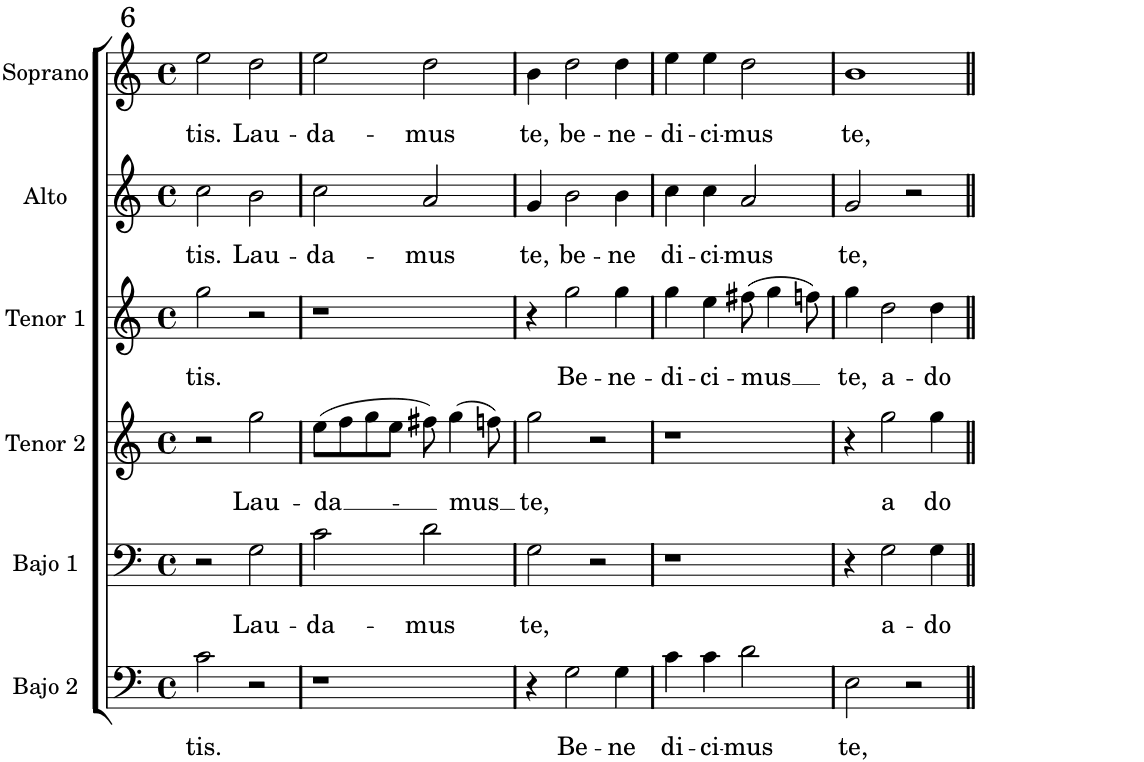
\includegraphics[angle=0, width=1\textwidth]{Ejemplo1.png}
\caption{\label{Ejemplo1}Compases del 6--10 del Gloria in Excelsis Deo.}
\end{figure}

Es importante mencionar que de todos ejemplos que se encontraron en la misa, las dos voces que se tomaron no siempre fueron las de soprano y alto ni tampoco fueron siempre voces adyacentes. Esto se puede ver claramente en el ejemplo 2, donde las voces que se tomaron fueron las de tenor 1 y bajo 1. 

Ahora bien, para codificar la obra en una matriz, se construyó una de tamaño $(32 \times 3) \times 18$, donde $32$ es el número de ejemplos encontrados en toda la misa, $18$ corresponde al ejemplo con el mayor número de intervalos de contrapunto ó $17=18-1$ transiciones -como se le quiera ver-, y $3$ viene de haber hecho lo siguiente: 

\begin{equation*}
M=\left(
\begin{array}{c c c c c c c c c c c c c c c c c c}
6 & 6 & 7 & 7 & 8 & 8 & 8 & 9 & 9 & 9 & 0 & 0 & 0 & 0 & 0 & 0 & 0 & 0 \\
4 & 2 & 4 & 2 & 11 & 2 & 2 & 4 & 4 & 2 & 0 & 0 & 0 & 0 & 0 & 0 & 0 & 0 \\
8 & 9 & 8 & 7 & 8 & 9 & 9 & 8 & 8 & 7 & 0 & 0 & 0 & 0 & 0 & 0 & 0 & 0 \\
\vdots & \vdots & \vdots & \vdots & \vdots & \vdots & \vdots & \vdots & \vdots & 
\vdots & \vdots & \vdots & \vdots & \vdots & \vdots & \vdots & \vdots 
\end{array} 
\right)
\end{equation*}
 
 Estos son los tres primeros renglones de la matriz $M$ que corresponden al ejemplo $1$. En el primer renglón se encuentran, escritos consecutivamente, los números de compás correspondientes a cada intervalo de contrapunto. En el segundo y tercer renglones se encuentran respectivamente los números $a$ y $b \in \mathbb{Z}_{12}$ de cada uno de los intervalos de contrapunto $a+\epsilon.b$. 
 
 Entonces, para cada ejemplo se tienen $3$ renglones en la matriz $M$. Cada ejemplo termina cuando aparecen columnas de $0$ a la izquierda del último intervalo de contrapunto. El único que no tiene columnas de $0$ es el que cuenta con el mayor número de transiciones: el ejemplo 25. De esta manera, aunque el compás donde se encuentra cada intervalo de contrapunto no es único, las dos entradas que ocupa en la matriz sí lo son. La obra completa codificada puede verse en el apéndice~\ref{Obra}.
 
 Se menciona que no se hallaron ejemplos en las partes de la obra correspondientes al Kyrie eleison y al Agnus Dei II. En los cuadros~\ref{Gloria}-\ref{Agnus} se puede ver en qué compases de las partes restantes se encontraron todos los ejemplos.  
 
\begin{table}[h]
\centering
\begin{tabular}{| c | c | c |}
\hline
\multicolumn{3}{|c|}{Gloria in excelsis Deo}\\
\hline
Ejemplo & Compases & Voces\\
\hline
$1$ & $6-9$ & Soprano y Alto\\
$2$ & $21-24$ & Tenor I y Bajo I\\
$3$ & $24-26$ & Soprano y Bajo II\\
$4$ & $28-31$ & Alto y Tenor I\\
$5$ & $32-34$ & Soprano y Alto\\
$6$ & $35-37$ & Alto y Bajo I\\
$7$ & $41-43$ & Soprano y Bajo I\\
$8$ & $63-65$ & Alto y Bajo I\\
$9$ & $67-72$ & Soprano y Alto\\
$10$ & $74-77$ & Soprano y Bajo II\\
\hline
\end{tabular}
\caption{\label{Gloria}Ejemplos 1-10.} 
\end{table}

\begin{table}[h]
\centering
\begin{tabular}{| c | c | c |}
\hline
\multicolumn{3}{|c|}{Credo in unum Deum}\\
\hline
Ejemplo & Compases & Voces\\
\hline
$11$ & $1-3$ & Alto y Tenor I\\
$12$ & $8-10$ & Alto y Soprano\\
$13$ & $20-24$ & Soprano y Bajo I\\
$14$ & $33-36$ & Soprano y Tenor I\\
$15$ & $43-45$ & Tenor I y Bajo I\\
$16$ & $52-54$ & Tenor I y Bajo I\\
$17$ & $60-62$ & Soprano y Bajo I\\
$18$ & $75-77$ & Alto y Tenor I\\
$19$ & $83-86$ & Alto y Tenor I\\
$20$ & $90-93$ & Tenor I y Bajo I\\
$21$ & $101-105$ & Soprano y Alto\\
$22$ & $101-106$ & Alto y Tenor II\\
$23$ & $122-125$ & Soprano y Bajo I\\
$24$ & $148-152$ & Soprano y Bajo I\\
\hline
\end{tabular}
\caption{\label{Credo}Ejemplos 11-24.}  
\end{table}

\begin{table}[h]
\centering
\begin{tabular}{| c | c | c |}
\hline
\multicolumn{3}{|c|}{Sanctus-Hosanna}\\
\hline
Ejemplo & Compases & Voces\\
\hline
$25$ & $17-20$ & Soprano y Bajo I\\
$26$ & $58-61$ & Soprano y Alto\\
$27$ & $58-60$ & Tenor II y Bajo I\\
$28$ & $62-64$ & Alto y Bajo I\\
\hline
\end{tabular}
\caption{\label{Sanctus}Ejemplos 25-28.}  
\end{table}

\begin{table}[h]
\centering
\begin{tabular}{| c | c | c |}
\hline
\multicolumn{3}{|c|}{Benedictus qui venit}\\
\hline
Ejemplo & Compases & Voces\\
\hline
$29$ & $1-3$ & Soprano y Tenor I\\
$30$ & $39-43$ & Soprano y Alto\\
$31$ & $40-42$ & Tenor II y Bajo I\\
\hline
\end{tabular}
\caption{\label{Benedictus}Ejemplos 29-31.} 
\end{table}

\begin{table}[h]
\centering
\begin{tabular}{| c | c | c |}
\hline
\multicolumn{3}{|c|}{Agnus Dei I}\\
\hline
Ejemplo & Compases & Voces\\
\hline
$32$ & $44-46$ & Alto y Tenor II\\
\hline
\end{tabular}
\caption{\label{Agnus}Ejemplo 32.} 
\end{table}

Finalmente queda decidir si en un ejemplo dado, de las dos voces que se tomaron, el cantus firmus se encuentra arriba y el discanto abajo o viceversa. Afortunadamente, por lo visto en la sección~\ref{Orientacion}, nuestra elección puede hacerse de acuerdo a nuestra conveniencia. Y es que como la obra primero será analizada con la teoría de Fux, en los casos en los que las reglas no se cumplían eligiendo al contrapunto barriente, entonces se escogió el colgante. Esto sólo sucedió en los ejemplos 1, 9, 14, 19, 23, 26 y 30, y en algunos de éstos, el número de compases analizados se redujo en uno. Esto sucedió con los ejemplos 19, 26 y 30.   

\subsection{El Análisis usando las reglas de Fux}

Las reglas de Fux\index{Fux} se cumplieron, en cuanto a transiciones, para casi todos los ejemplos, a excepción de los siguientes: 1, 8, 9, 10, 13, 16, 19, 24 y 25. En todos ellos la regla no se cumplió porque se usó un movimiento no permitido: el movimiento directo a una consonancia perfecta. Lo cierto es que en varios casos el movimiento no permitido apareció en la última transición, de modo que si no se toma en cuenta el último intervalo, la regla deja de no cumplirse; en otras palabras, si se eliminara la última transición de los ejemplos donde esto sucedió, la regla se cumpliría en $5$ transiciones más de las $15$ en las que no se cumplía. En el cuadro~\ref{Faltas} puede verse en qué transiciones no se cumplieron las reglas de Fux. El asterisco indica que se trata de la última transición.

\begin{table}[h]
\centering
\begin{tabular}{| c | c | c | c | c | c |}
\hline
Ejemplo & \multicolumn{2}{c|}{Transición} & Ejemplo & \multicolumn{2}{c|}{Transición}\\
\hline
$1$ & $4$   &    & $13$ & $8$ &  \\
        & $10$ & * &           & $14$ & \\
\hline
$8$ & $5$  &      & $16$ & $2$ & \\
        & $6$  &  *  &            & $6$ & *\\
\hline
$9$ & $9$   &  &  $19$ & $8$ & \\ \cline{4-6}
        & $18$ & *& $24$ & $5$ & \\
\hline
$10$ & $10$ & * & $25$ &  $4$ &\\
          &            &   &            & $6$  & \\
\hline
\end{tabular}
\caption{\label{Faltas}Transiciones donde se infringieron las reglas de Fux.}
\end{table}
 
\subsection{El Análisis usando el Teorema de Contrapunto}

Para llevar a cabo este análisis, se usó la tabla de sucesores admisibles del Teorema~\ref{TC}. Para cada ejemplo, en cada transición de $a_i+ \epsilon.b_i$ a $a_{i+1}+\epsilon.b_{i+1}$, se buscó la consonancia correspondiente a $b_i$, y para todas las simetrías de ésta, si $b_{i+1}$ pertenecía al menos a un conjunto de sucesores admisibles. Como se mencionó anteriormente, se escribió un programa en Matlab para llevar a cabo esta tarea. El programa se encuentra en el apéndice~\ref{Programa}. Cabe señalar que cuando se tiene un cantus firmus $x\neq 0$, existe un teorema que garantiza que después de haber encontrado los sucesores admisibles para un cantus firmus igual a cero, basta trasladarlos con $e^x$ \cite{TesisOctavio}.

Los resultados fueron los siguientes. En total se analizaron $203$ transiciones, de las $250$ existentes. La razón se debe a que sólo en $203$ hubo una transición de un intervalo de contrapunto a otro consecutivo y \emph{diferente}. Es evidente que lo mismo sucedió para el análisis usando las reglas de Fux, por lo que también lo es que en el ejemplo $12$ haya una disonancia en el intervalo de contrapunto número $2$.  En el cuadro~\ref{Simetrias1} puede verse en cuántas transiciones media cada simetría de contrapunto. En el cuadro~\ref{Simetrias2} se encuentra la información de cuántas transiciones tuvieron de una a cinco simetrías o si de hecho no existió simetría alguna. Finalmente, en el cuadro~\ref{NoSimetrias} se puede ver para qué ejemplos y en qué transiciones no existieron simetrías de contrapunto. El total de transiciones en donde no hubo simetría es $6$.

\begin{table}[h]
\centering
\begin{tabular}{| c | c |}
\hline
Simetría & Frecuencia\\
\hline
$e^{\epsilon{.}6}\circ (1+\epsilon{.}6)$ & $71$\\
$e^{\epsilon{.}6}\circ (7+\epsilon{.}6)$ & $62$\\
$e^{\epsilon{.}11}\circ(11+\epsilon{.}8)$& $14$\\
$e^{\epsilon{.}11}\circ(11+\epsilon{.}4)$ & $15$\\
$e^{\epsilon{.}11}\circ 11$ & $17$\\
$e^{\epsilon{.}8}\circ (5+\epsilon{.}8)$ & $60$\\
$e^{\epsilon{.}8}\circ (5+\epsilon{.}4)$ & $62$\\
$e^{0}\circ 7$ & $37$\\
$e^{\epsilon{.}3}\circ 7$ & $16$\\
$e^{\epsilon{.}3}\circ (7+\epsilon{.}4)$ & $21$\\
$e^{\epsilon{.}3}\circ(7+\epsilon{.}8)$ & $17$\\
\hline
\end{tabular}
\caption{\label{Simetrias1}Distribución de cada una de las simetrías de contrapunto de la misa.}
\end{table}           

\begin{table}[h]
\centering
\begin{tabular}{| l  c |}
\hline
Transiciones: & 203\\
\hline
Con cinco simetrías: & $6$ \\
Con cuatro simetrías: & $20$ \\
Con tres simetrías: & $4$ \\
Con dos simetrías: & $103$ \\
Con una simetría: & $64$ \\
Sin simetría: & $6$ \\
\hline
\end{tabular}
\caption{\label{Simetrias2}Transiciones con 0, 1, 2, 3, 4 ó 5 simetrías.}
\end{table}   

\begin{table}[h]
\centering
\begin{tabular}{| c | c |}
\hline
Ejemplo & Transición \\
\hline
$5$ & $6$ \\
$7$ & $7$ \\
$17$ & $4$ \\
$20$ & $1$ \\
$22$ & $5$ \\
$29$ & $9$ \\
\hline
\end{tabular}
\caption{\label{NoSimetrias}Ejemplos donde no hubo simetría.}
\end{table}  

Si de acuerdo al Teorema de Contrapunto se toman en cuenta todas las transiciones de intervalos de contrapunto posibles, existen un total de 5112, omitiendo las de un intervalo en sí mismo. De éstas, 528 están prohibidas y hay 1248, 2280, 96, 576 y 384 con 1, 2, 3, 4 y 5 simetrías respectivamente \cite{TesisOctavio}. La media de estos datos es  $\mu_{TC}=2{.}0188$, la desviación estándar $\sigma_{TC}=1{.}3427$, la mediana es $q_{50,TC}=2$, el coeficiente de asimetría $sk_{TC}={.}7341$ y la curtosis es $k_{TC}=2{.}9750$ (platicúrtica). Para los ejemplos analizados en la misa, como se esperaría por la distribución del número de simetrías por transición del Teorema de Contrapunto, la media es $\mu_M=1{.}9310$ y la mediana es $q_{50,M}=2$. Lo sorprendente es que el coeficiente de asimetría sea $sk_{M}=1{.}1$, que la curtosis sea $k_M=4{.}1508$ y la desviación estándar $\sigma_M=1{.}0555$. Es decir, la distribución en el caso de la misa es más asimétrica (cargada hacia la izquierda) y de hecho más concentrada alrededor de la media (por ser leptocúrtica y con una desviación estándar menor a la del caso general). Una gráfica de las tablas de frecuencias se puede ver en la figura~\ref{Frecuencias}. Lo cierto es que con estos datos se puede ver que hay una concentración aún mayor en transiciones que se explican con dos o una simetría de lo que se esperaría si los intervalos de las transiciones fueran escogidos aleatoriamente. Si se piensa nuevamente que en Física las simetrías locales son responsables de la aparición de fuerzas, entonces a mayor número de simetrías, hay una mayor disipación de las fuerzas. 

\begin{figure}[h]
\centering
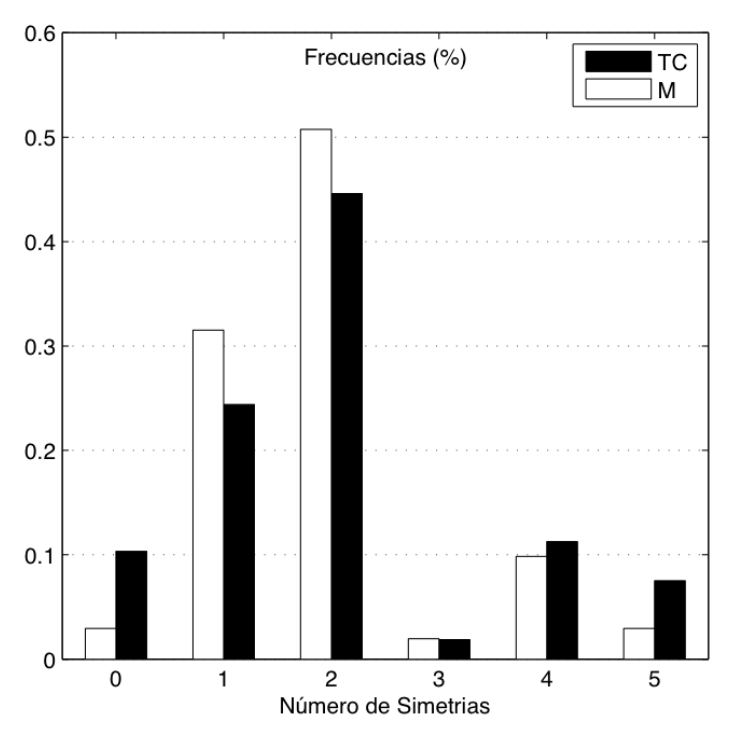
\includegraphics[angle=0, width=0.5\textwidth]{Frecuencias.png}
\caption{\label{Frecuencias}Distribución de las simetrías del Teorema de Contrapunto (TC) y de la Misa del Papa Marcelo (M).}
\end{figure}

\appendix

\chapter{La Obra Codificada}\label{Obra}
\begin{table}[h]
\centering
{\tiny
\begin{tabular}{ c c c c c c c c c c c c c c c c c c c}
& 0 & 1 & 2 & 3 & 4 & 5 & 6 & 7 & 8 & 9 & 10 & 11 & 12 & 13 & 14 & 15 & 16 & 17 \\ 
%Gloria in Excelsis Deo
1 & 6 & 6 & 7 & 7 & 8 & 8 & 8 & 9 & 9 & 9 & 0 & 0 & 0 & 0 & 0 & 0 & 0 & 0 \\ %1
 & 4 & 2 & 4 & 2 & 11 & 2 & 2 & 4 & 4 & 2 & 0 & 0 & 0 & 0 & 0 & 0 & 0 & 0 \\ %2
 & 8 & 9 & 8 & 7 & 8 & 9 & 9 & 8 & 8 & 7 & 0 & 0 & 0 & 0 & 0 & 0 & 0 & 0 \\%3
2 & 21 & 21 & 21& 22 & 22 & 22 & 23 & 23 & 23 & 23 & 23 & 23 & 23 & 24 & 0 & 0 & 0 & 0\\%4
 & 0 & 0 & 11 & 0 & 9 & 2 & 0 & 0 & 11 & 9 & 11 & 0 & 9 & 2 & 0 & 0 & 0 & 0 \\ %5
 & 4 & 4 & 3 & 4 & 3 & 3 & 4 & 4 & 3 & 3 & 3 & 4 & 3 & 7 & 0 & 0 & 0 & 0 \\ %6 
3 & 24 & 24 & 25 & 25 & 25 & 26 & 26 & 26 & 26 & 0 & 0 & 0 & 0 & 0 & 0 & 0 & 0 & 0 \\  %7
 & 7 & 6 & 7 & 4 & 9 & 7 & 0 & 2 & 7 & 0 & 0 & 0 & 0 & 0 & 0 & 0 & 0 & 0 \\  %8 
 & 4 & 3 & 4 & 3 & 3 & 4 & 3 & 4 & 4 & 0 & 0 & 0 & 0 & 0 & 0 & 0 & 0 & 0 \\  %9 
4 & 28 & 29 & 29 & 29 & 29 & 30 & 31& 0 & 0 & 0 & 0 & 0 & 0 & 0 & 0 & 0 & 0 & 0 \\  %10 
 & 9 & 7 & 0 & 0 & 0 & 0 & 0 & 0 & 0 & 0 & 0 & 0 & 0 & 0 & 0 & 0 & 0 & 0 \\  %11
 & 8 & 9 & 7 & 7 & 7 & 9 & 7 & 0 & 0 & 0 & 0 & 0 & 0 & 0 & 0 & 0 & 0 & 0 \\  %12
5 & 32 & 32 & 32 & 32 & 32 & 33 & 33 & 34 & 0 & 0 & 0 & 0 & 0 & 0 & 0 & 0 & 0 & 0 \\  %13
 & 7 & 2 & 2 & 7 & 7 & 5 & 9 & 9 & 0 & 0 & 0 & 0 &  0 & 0 & 0 & 0 & 0 & 0 \\  %14
 & 4 & 0 & 0 & 9 & 9 & 4 & 8 & 7 & 0 & 0 & 0 & 0 & 0 & 0 & 0 & 0 & 0 & 0 \\  %15
6 & 35 & 36 & 36 & 37 & 0 & 0 & 0 & 0 & 0 & 0 & 0 & 0 & 0 & 0 & 0 & 0 & 0 & 0 \\  %16
 & 2 & 9 & 2 &10 & 0 & 0 & 0 & 0 & 0 & 0 & 0 & 0 & 0 & 0 & 0 & 0 & 0 & 0 \\  %17
 & 7 & 0 & 7 & 8 & 0 & 0 & 0 & 0 & 0 & 0 & 0 & 0 & 0 & 0 & 0 & 0 & 0 & 0 \\  %18
7 & 41 & 41 & 41 & 42 & 42 & 42 & 43 & 43 & 0 & 0 & 0 & 0 & 0 & 0 & 0 & 0 & 0 & 0 \\  %19 
 & 9 & 9 & 9 & 0 & 11 & 9 & 7 & 5 & 0 & 0 & 0 & 0 & 0 & 0 & 0 & 0 & 0 & 0 \\  %20
 & 7 & 7 & 7 & 4 & 3 & 3 & 4 & 4 & 0 & 0 & 0 & 0 & 0 & 0 & 0 & 0 & 0 & 0 \\  %21
8 & 63 & 63 & 63 & 64 & 64 & 65 & 0 & 0 & 0 & 0 & 0 & 0 & 0 & 0 & 0 & 0 & 0 & 0 \\  %22
 & 0 & 7 & 0 & 5 & 0 & 0 & 0 & 0 & 0 & 0 & 0 & 0 & 0 & 0 & 0 & 0 & 0 & 0 \\  %23
 & 7 & 0 & 7 & 4 & 7 & 0 & 0 & 0 & 0 & 0 & 0 & 0 & 0 & 0 & 0 & 0 & 0 & 0 \\  %24
9 & 67 & 67& 67 & 68 & 68 & 68 & 68 & 69 & 69 & 70 & 70 & 70 & 71 & 71 & 71 & 71 & 72 & 72 \\ %25
 & 7 & 11 & 11 & 0 & 7 & 9 & 11 & 0 & 9 & 7 & 11 & 11 & 0 & 7 & 9 & 11 & 0 & 9 \\ %26
 & 8 & 9 & 9 & 8 & 3 & 9 & 9 & 8 & 7 & 8 & 9 & 9 & 8 & 3 & 9 & 9 & 8 & 7 \\  %27
10 & 74 & 74 & 74 & 75 & 75 & 75 & 75 & 76 & 76 & 77 & 0 & 0 & 0 & 0 & 0 & 0 & 0 & 0 \\ %28 
 & 0 & 11 & 0 & 11 & 7 & 9 & 11 & 0 & 5 & 0 & 0 & 0 & 0 & 0 & 0 & 0 & 0 & 0 \\ %29
 & 4 & 3 & 4 & 3 & 4 & 3 & 3 & 7 & 4 & 7 & 0 & 0 & 0 & 0 & 0 & 0 & 0 & 0 \\ %30
%Credo in unum Deo
11 & 1 & 2 & 2 & 3 & 3 & 0 & 0 & 0 & 0 & 0 & 0 & 0 & 0 & 0 & 0 & 0 & 0 & 0 \\ %31
 & 2 & 2 & 2 & 4 & 2 & 0 & 0 & 0 & 0 & 0 & 0 & 0 & 0 & 0 & 0 & 0 & 0 & 0 \\  %32
 & 7 & 7 & 7 & 9 & 7 & 0 & 0 & 0 & 0 & 0 & 0 & 0 & 0 & 0 & 0 & 0 & 0 & 0 \\  %33
12 & 8 & 8 & 9 & 9 & 9 & 10 & 10 & 0 & 0 & 0 & 0 & 0 & 0 & 0 & 0 & 0 & 0 & 0 \\ %34
 & 7 & 7 & 7 & 7 & 4 & 9 & 9 & 0 & 0 & 0 & 0 & 0 & 0 & 0 & 0 & 0 & 0 & 0 \\ %35
 & 5 & 5 & 7 & 7 & 0 & 8 & 8 & 0 & 0 & 0 & 0 & 0 & 0 & 0 & 0 & 0 & 0 & 0 \\ %36
13 & 20 & 20 & 21 & 21 & 21& 22 & 22 & 22 & 22 & 22 & 23 & 23 & 23 & 23 & 24 & 0 & 0 & 0 \\ %37
 & 2 & 2 & 2 & 2 & 5 & 0 & 0 & 7 & 9 & 9 & 7 & 9 & 7 & 2 & 7 & 0 & 0 & 0 \\ %38
 & 0 & 0 & 3 & 3 & 0 & 4 & 4 & 7 & 3 & 3 & 4 & 7 & 4 & 7 & 4 & 0 & 0 & 0 \\ %39
14 & 33 & 33 & 33 & 34 & 34 & 34 & 35 & 35 & 35 & 36 & 36 & 0 & 0 & 0 & 0 & 0 & 0 & 0 \\ %40
 & 0 & 7 & 7 & 4 & 4 & 0 & 2 & 4 & 2 & 0 & 11 & 0 & 0 & 0 & 0 & 0 & 0 & 0 \\ %41
 & 0 & 9 & 7 & 8 & 7 & 0 & 9 & 8 & 9 & 9 & 8 & 0 & 0 & 0 & 0 & 0 & 0 & 0 \\ %42
\end{tabular}
}
\caption{Matriz $M$ con un renglón (transición) y una columna (ejemplo) adicionales para su rápida localización.}
\end{table}


\begin{table}
{\tiny
\centering
\begin{tabular}{c c c c c c c c c c c c c c c c c c c}
& 0 & 1 & 2 & 3 & 4 & 5 & 6 & 7 & 8 & 9 & 10 & 11 & 12 & 13 & 14 & 15 & 16 & 17 \\ 
15 & 43 & 43 & 43 & 44 & 44 & 45 & 0 & 0 & 0 & 0 & 0 & 0 & 0 & 0 & 0 & 0 & 0 & 0 \\ %43
 & 2 & 7 & 0 & 2 & 9 & 2 & 0 & 0 & 0 & 0 & 0 & 0 & 0 & 0 & 0 & 0 & 0 & 0 \\ %44
 & 4 & 0 & 7 & 3 & 7 & 0 & 0 & 0 & 0 & 0 & 0 & 0 & 0 & 0 & 0 & 0 & 0 & 0 \\ %45
16 & 52 & 52 & 53 & 53 & 54 & 54 & 0 & 0 & 0 & 0 & 0 & 0 & 0 & 0 & 0 & 0 & 0 & 0 \\ %46
 & 11 & 0 & 9 & 5 & 7 & 0 & 0 & 0 & 0 & 0 & 0 & 0 & 0 & 0 & 0 & 0 & 0 & 0 \\ %47
 & 8 & 7 & 8 & 0 & 9 & 7 & 0 & 0 & 0 & 0 & 0 & 0 & 0 & 0 & 0 & 0 & 0 & 0 \\ %48
17 & 60 & 60 & 60 & 61 & 61 & 62 & 62 & 0 & 0 & 0 & 0 & 0 & 0 & 0 & 0 & 0 & 0 & 0  \\%49
 & 7 & 9 & 11 & 0 & 0 & 11 & 0 & 0 & 0 & 0 & 0 & 0 & 0 & 0 & 0 & 0 & 0 & 0 \\ %50
 & 4 & 3 & 3 & 4 & 0 & 3 & 0 & 0 & 0 & 0 & 0 & 0 & 0 & 0 & 0 & 0 & 0 & 0 \\ %51
18 & 75 & 75 & 75 & 75 & 76 & 76 & 76 & 76 & 77 & 77 & 77 & 0 & 0 & 0 & 0 & 0 & 0 & 0 \\ %52
 & 2 & 9 & 9 & 9 & 9 & 4 & 7 & 5 & 4 & 2 & 0 & 0 & 0 & 0 & 0 & 0 & 0 & 0 \\ %53
 & 0 & 8 & 8 & 8 & 7 & 8 & 9 & 9 & 8 & 9 & 9 & 0 & 0 & 0 & 0 & 0 & 0 & 0 \\ %54
19 & 83 & 83 & 83 & 83 & 84 & 84 & 84 & 85 & 85 & 85 & 85 & 86 & 0 & 0 & 0 & 0 & 0 & 0 \\ %55
 & 5 & 5 & 4 & 2 & 4 & 0 & 2 & 9 & 4 & 4 & 4 & 4 & 0 & 0 & 0 & 0 & 0 & 0 \\ %56
 & 4 & 4 & 3 & 7 & 3 & 4 & 3 & 7 & 3 & 3 & 3 & 3 & 0 & 0 & 0 & 0 & 0 & 0 \\ %57
20 & 90 & 90 & 91 & 91 & 92 & 92 & 92 & 93 & 93 & 93 & 93 & 93 & 0 & 0 & 0 & 0 & 0 & 0 \\ %58
 & 0 & 4 & 5 & 0 & 0 & 0 & 11 & 0 & 11 & 7 & 9 & 11 & 0 & 0 & 0 & 0 & 0 & 0 \\ %59
 & 4 & 0 & 7 & 0 & 0 & 4 & 3 & 4 & 3 & 4 & 3 & 3 & 0 & 0 & 0 & 0 & 0 & 0 \\%60
21 & 01 & 01 & 02 & 02 & 03 & 03 & 03 & 04 & 04 & 05 & 0 & 0 & 0 & 0 & 0 & 0 & 0 & 0 \\ %61
 & 7 &  7 &  7 &  7  & 3 &  7 &  7 &  7 &  7 &  9 &  0  & 0 & 0 & 0 & 0 & 0 & 0 & 0 \\ %62
 & 7 &  7 &  7 &  7 &  0 &  9 &  9 &  9  & 9 &  3  & 0 & 0 & 0 & 0 & 0 & 0 & 0 & 0 \\ %63
22 & 01 & 01 & 02 & 02 & 03 & 03 & 03 & 04 & 04 & 05 & 05 & 05 & 06 & 0 & 0 & 0 & 0 & 0 \\ %64
 & 7 & 7 & 7 & 7 & 4 & 7 & 7 & 7 & 7 & 9 & 9 & 9 & 9 & 0 & 0 & 0 & 0 & 0 \\%65
 & 7 & 7 & 7 & 7 & 3 & 9 & 9 & 9 & 9 & 8 &  8 &  8 &  8 &  0 &  0 & 0 &  0 & 0 \\ %66
23 & 22 & 22 & 23 & 23 & 23 & 24 & 24 & 24 & 24 & 24 & 25 & 0 & 0 & 0 & 0 & 0 & 0 & 0 \\ %67
 & 0 & 11 & 9 &  7 &  5 &  4 &  4 &  0 &  2 & 2 & 4 & 0 & 0 & 0 & 0 & 0 & 0 & 0 \\ %68
 & 9 &  8 &  8 &  9 &  9 &  8 &  8 &  0 &  7 & 9 & 8 & 0 & 0 & 0 & 0 & 0 & 0 & 0 \\ %69
24 & 48 & 48 & 48 & 49 & 50 & 50 & 50 & 51 & 51 & 51 & 52 & 0 & 0 & 0 & 0 & 0 & 0 & 0 \\ %70
 & 0 &  0 &  0 &  7 &  0 &  0 & 11 & 9 &  7 &  5 &  0 &  0 &  0 & 0 &  0 &  0 &  0 &  0 \\ %71
 & 0 &  4 &  4  & 7 &  0 &  4 & 3 &  3 &  4 &  4 &  7  & 0 &  0 &  0 &  0 &  0 &  0 &  0 \\ %72

%Sanctus-Hosanna
25 & 17 & 17 & 18 & 18 & 19 & 19 & 20 & 0 & 0 & 0 & 0 & 0 & 0 & 0 & 0 & 0 & 0 & 0 \\ %73    
 & 7 & 0 & 9 & 2 & 7 & 0 & 5 & 0 & 0 & 0 & 0 & 0 & 0 & 0 & 0 & 0 & 0 & 0 \\ %74
 & 7 & 4 & 3 & 0 & 4 & 0 & 7 & 0 & 0 & 0 & 0 & 0 & 0 & 0 & 0 & 0 & 0 & 0 \\ %75
26 & 58 & 59 & 59 & 60 & 60 & 61 & 0 & 0 & 0 & 0 & 0 & 0 & 0 & 0 & 0 & 0 & 0 & 0 \\ %76 
 & 11 & 0 & 0 & 2 &  2 & 2 & 0 &  0 & 0 & 0 & 0 & 0 & 0 & 0 & 0 & 0 & 0 & 0 \\ %77
 & 8 & 7 & 9 & 7 & 9 & 7 & 0 & 0 & 0 & 0 & 0 & 0 & 0 & 0 & 0 & 0 & 0 & 0 \\%78
27 & 58 & 59 & 59 & 60 & 60 & 0 & 0 & 0 & 0 & 0 & 0 & 0 & 0 & 0 & 0 & 0 & 0 & 0 \\ %79
 & 7 & 0 & 9 & 2 & 7 & 0 & 0 & 0 & 0 & 0 & 0 & 0 & 0 & 0 & 0 & 0 & 0 & 0 \\ %80
 & 7 & 4 & 7 & 3 & 0 & 0 & 0 & 0 & 0 & 0 & 0 & 0 & 0 & 0 & 0 & 0 & 0 & 0 \\ %81
28 & 62 & 62 & 63 & 64 & 0 & 0 & 0 & 0 & 0 & 0 & 0 & 0 & 0 & 0 & 0 & 0 & 0 & 0 \\ %82
 & 11& 0 & 9 & 2 & 0 & 0 & 0 & 0 & 0 & 0 & 0 & 0 & 0 & 0 & 0 & 0 & 0 & 0 \\ %83
 & 8 & 4 & 0 & 3 & 0 & 0 &  0 & 0 & 0 & 0 & 0 & 0 & 0 & 0 & 0 & 0 & 0 & 0 \\ %84  
%Benedictus qui venit
29 & 1 & 2 & 3 & 3 & 3 & 3 & 3 & 0 & 0 & 0 & 0 & 0 & 0 & 0 & 0 & 0 & 0 & 0 \\ %85   
 & 7 & 9 & 11 & 9 & 11 & 0 &  2 & 0 & 0 & 0 & 0 & 0 & 0 & 0 & 0 & 0 & 0 & 0 \\ %86
 & 0 & 8 & 8 & 8 & 3 & 4 & 3 & 0 & 0 & 0 & 0 & 0 & 0 & 0 & 0 & 0 & 0 & 0 \\ %87
30 & 39 & 40 & 41 & 41 & 42 & 42 & 43 & 0 & 0 & 0 & 0 & 0 & 0 & 0 & 0 & 0 & 0 & 0 \\ %88
 & 11 & 11& 7 & 9 & 9 & 11 & 9 & 0 & 0 & 0 & 0 & 0 & 0 & 0 & 0 & 0 & 0 & 0 \\ %89
 & 8 & 8 & 7 & 9 & 7 & 9 & 7 & 0 & 0 & 0 & 0 & 0 & 0 & 0 & 0 & 0 & 0 & 0 \\ %90
31 & 40 & 41 & 41 & 42 & 42 & 0 &  0 & 0 & 0 & 0 & 0 & 0 & 0 & 0 & 0 & 0 & 0 & 0 \\ %91
 & 7 & 0 & 9 & 2 & 7 & 0 & 0 & 0 & 0 & 0 & 0 & 0 & 0 & 0 & 0 & 0 & 0 & 0 \\ %92
 & 7 & 4 & 7 & 3 & 0 & 0 & 0 & 0 & 0 & 0 & 0 & 0 & 0 & 0 & 0 & 0 & 0 & 0 \\ %93
%Agnus Dei I
32 & 44 & 44 & 44 & 44 & 44 & 44 & 44 & 44 & 45 & 46 & 0 & 0 & 0 & 0 & 0 & 0 & 0 & 0 \\%94
 & 9 & 7 & 9 & 11 & 0 & 11 & 9 & 7 & 9 & 7 & 0 & 0 & 0 & 0 & 0 & 0 & 0 & 0 \\%95
 & 8 & 9 & 8 & 8 & 9 & 8 & 8 & 9 & 8 & 9 & 0 & 0 & 0 & 0 & 0 & 0 & 0 & 0 \\ %96
\end{tabular}
}
\end{table}

 
\chapter{El Programa}\label{Programa} 

{\tiny
\begin{verbatim}
function[]=contrapunto(A)
%A es la matriz de mxn donde se encuentra codificada la obra. 
%Consta de rx3 renglones, donde r=32 indica el numero de ejemplos
%extraidos de la obra

%La informacion por cada 3 renglones es como sigue:
%En el primero aparece el numeros de compas donde se ubica cada intervalo 
%de contrapunto del ejemplo
%Si a+epsilon.b cambia a a'+epsilon.b' se tiene (i son los renglones y 
%j las columnas):

% 1       j-1 j
 
%   . . .  c  c' . . . c'' 0 . . . 0     i
%   . . .  a  a' . . . a'' 0 . . . 0     i+1  
%   . . .  b  b' . . . b'' 0 . . . 0     i+2 

%El ejemplo termina antes del primer compas igual a 0

[m,n]=size(A);
K=[0,3,4,7,8,9];
D=[1,2,5,6,10,11];
Z12par=[0,2,4,6,8,10];
Z12impar=[1,3,5,7,9,11];
Z12=[Z12par,Z12impar];

k0=0; %cuenta, para una transicion, cuantas simetrias hay: 0,1,2,3,4 o 5
j=1; %se empieza en la primera columna

%De s1 a s11 se tienen las simetrias en orden de aparicion en la tesis
%s1=[6 0 1;0 6 6]; s2=[6 0 7;0 6 6]; s3=[11 0 11;0 11 8]; s4=[11 0 11;0 11 4];
%s5=[11 0 11;0 11 0]; s6=[8 0 5;0 8 8]; s7=[8 0 5;0 8 4]; s8=[0 0 7;0 0 0];
%s9=[3 0 7;0 3 0]; s10=[3 0 7;0 3 4]; s11=[3 0 7;0 3 8];

%En los conjuntos Si se guardan los (k,j) correspondientes a la simetria si,
%donde k corresponde al numero de ejemplo y j al numero de transicion.
%Es decir, si en el ejemplo k, de a+epsilon.b en la columna j se 
%cambia a a'+epsilon.b' en la columna j+1 con simetria si, (k,j) se guarda
%en Si

%NS.- conjunto de las (k,j) para los cuales no hubo 
%sucesor admisible de acuerdo al Teorema de Contrapunto

%D.- conjunto de las (k,j) de las transiciones que son una disonancia

%Uno, Dos, Tres, Cuatro, Cinco contienen a las (k,j) 
%correspondientes a una simetria, dos simetrias, etc.

S1=[]; S2=[]; S3=[]; S4=[]; S5=[]; S6=[]; S7=[]; S8=[]; S9=[]; S10=[]; S11=[]; NS=[]; D=[];
Uno=[]; Dos=[]; Tres=[]; Cuatro=[]; Cinco=[]; 

%En este ciclo se analiza si cada transicion es o no un sucesor admisible. Si
%lo es se guarda el vector (k,j) en todas las Si que correspondan. Si no, se 
%guarda en NS o en D

transiciones=0; %cuenta el total de transiciones en toda la obra
notransiciones=0;

for i=2:3:m-1
    j=1;
    while j<n & A(i-1,j)>0 & A(i-1,j+1)>0 %la condicion de paro ocurre
        %cuando aparece el primer compas igual a 0
        if ( A(i,j)~=A(i,j+1) | A(i+1,j)~=A(i+1,j+1) ) & find(K==A(i+1,j))>0
        % Si esta condicion no se cumpliera, no habria una verdadera transicion 
            if A(i+1,j)==0 %b'=0 de epsion.b'
                k0=0; 
                if (  (find( mod(A(i,j)+Z12par,12)==A(i,j+1) )>0 & find( [3,9]==A(i+1,j+1) )>0) | 
                (find( mod(A(i,j)+Z12impar,12)==A(i,j+1) )>0 & find( K==A(i+1,j+1) )>0)  )
                    S1=[S1,[(i+1)/3;j]];
                    k0=k0+1;
                end    
                if (  (find( mod(A(i,j)+Z12par,12)==A(i,j+1) )>0 & find( [3,7,9]==A(i+1,j+1) )>0) | 
                (find( mod(A(i,j)+Z12impar,12)==A(i,j+1) )>0 & find( setdiff(K,[7])==A(i+1,j+1) )>0)  )
                    S2=[S2,[(i+1)/3;j]];
                    k0=k0+1;
                end    
                if (  (find( mod(A(i,j)+[0,3,6,9],12)==A(i,j+1) )>0 & find( [3,4,7,8]==A(i+1,j+1) )>0) | 
                (find( mod(A(i,j)+[1,4,7,10],12)==A(i,j+1) )>0 & find( [0,3,7,8]==A(i+1,j+1) )>0) | 
                (find( mod(A(i,j)+[2,5,8,11],12)==A(i,j+1) )>0 & find( [0,3,4,7]==A(i+1,j+1) )>0)  ) 
                    S3=[S3,[(i+1)/3;j]];
                    k0=k0+1;   
                end
                if (  (find( mod(A(i,j)+[0,3,6,9],12)==A(i,j+1) )>0 & find( [3,4,7,8]==A(i+1,j+1) )>0) | 
                (find( mod(A(i,j)+[1,4,7,10],12)==A(i,j+1) )>0 & find( [0,3,4,7]==A(i+1,j+1) )>0) | 
                (find( mod(A(i,j)+[2,5,8,11],12)==A(i,j+1) )>0 & find( [0,3,7,8]==A(i+1,j+1) )>0)  ) 
                    S4=[S4,[(i+1)/3;j]];
                    k0=k0+1;
                end
                if find( [3,4,7,8]==A(i+1,j+1) )>0
                    S5=[S5,[(i+1)/3;j]];
                    k0=k0+1;       
                end    
                if k0==0
                    NS=[NS,[(i+1)/3;j]];
                elseif k0==1
                    Uno=[Uno,[(i+1)/3;j]];
                elseif k0==2
                    Dos=[Dos,[(i+1)/3;j]]; 
                elseif k0==3
                    Tres=[Tres,[(i+1)/3;j]];
                elseif k0==4
                    Cuatro=[Cuatro,[(i+1)/3;j]];
                else
                    Cinco=[Cinco,[(i+1)/3;j]];
                end
            end    
            if A(i+1,j)==3 %b'=3 de epsion.b'
                k3=0;
                if (   (find( mod(A(i,j)+[0,3,6,9],12)==A(i,j+1) )>0 & find( [0,4,7,8]==A(i+1,j+1) )>0) | 
                (find( mod(A(i,j)+[1,4,7,10],12)==A(i,j+1) )>0 & find( setdiff(K,[7])==A(i+1,j+1) )>0) | 
                (find( mod(A(i,j)+[2,5,8,11],12)==A(i,j+1) )>0 & find( setdiff(K,[9])==A(i+1,j+1) )>0) )
                    S6=[S6,[(i+1)/3;j]];
                    k3=k3+1;
                end
                if ( (find( mod(A(i,j)+[0,3,6,9],12)==A(i,j+1) )>0 & find( [0,4,7,8]==A(i+1,j+1) )>0) | 
                (find( mod(A(i,j)+[1,4,7,10],12)==A(i,j+1) )>0 & find( setdiff(K,[9])==A(i+1,j+1) )>0) | 
                (find( mod(A(i,j)+[2,5,8,11],12)==A(i,j+1) )>0 & find( setdiff(K,[7])==A(i+1,j+1) )>0) ) 
                    S7=[S7,[(i+1)/3;j]];
                    k3=k3+1;
                end
                if k3==0
                    NS=[NS,[(i+1)/3;j]];
                elseif k3==1
                    Uno=[Uno,[(i+1)/3;j]];
                else 
                    Dos=[Dos,[(i+1)/3;j]]; 
                end 
            end    
            if A(i+1,j)==4 %b'=4 de epsion.b'
                k4=0;
                if ( (find( mod(A(i,j)+Z12par,12)==A(i,j+1) )>0 & find( [3,9]==A(i+1,j+1) )>0) | 
                (find( mod(A(i,j)+Z12impar,12)==A(i,j+1) )>0 & find( K==A(i+1,j+1) )>0) )
                    S1=[S1,[(i+1)/3;j-1]];
                    k4=k4+1;
                end    
                if ( (find( mod(A(i,j)+Z12par,12)==A(i,j+1) )>0 & find( [3,7,9]==A(i+1,j+1) )>0) | 
                (find( mod(A(i,j)+Z12impar,12)==A(i,j+1) )>0 & find( setdiff(K,[7])==A(i+1,j+1) )>0) )
                    S2=[S2,[(i+1)/3;j]];
                    k4=k4+1;
                end
                if k4==0
                    NS=[NS,[(i+1)/3;j]];
                elseif k4==1
                    Uno=[Uno,[(i+1)/3;j]];
                else 
                    Dos=[Dos,[(i+1)/3;j]]; 
                end 
            end    
            if A(i+1,j)==7 %b'=7 de epsion.b'
                k7=0;
                if find( setdiff(K,[7])==A(i+1,j+1) )>0
                    S8=[S8,[(i+1)/3;j]];
                    k7=k7+1;
                end
                if k7==0
                    NS=[NS,[(i+1)/3;j]];
                else
                    Uno=[Uno,[(i+1)/3;j]];
                end   
            end    
            if A(i+1,j)==8 %b'=8 de epsion.b'
                k8=0;
                if find( [0,3,4,7]==A(i+1,j+1) )>0
                    S9=[S9,[(i+1)/3;j]];
                    k8=k8+1;
                end
                if ( (find( mod(A(i,j)+Z12par,12)==A(i,j+1) )>0 & find( [3,9]==A(i+1,j+1) )>0) | 
                (find( mod(A(i,j)+Z12impar,12)==A(i,j+1) )>0 & find( K==A(i+1,j+1) )>0) )
                    S1=[S1,[(i+1)/3;j]];
                    k8=k8+1;
                end    
                if ( (find( mod(A(i,j)+Z12par,12)==A(i,j+1) )>0 & find( [3,7,9]==A(i+1,j+1) )>0) | 
                (find( mod(A(i,j)+Z12impar,12)==A(i,j+1) )>0 & find( setdiff(K,[7])==A(i+1,j+1) )>0) )
                    S2=[S2,[(i+1)/3;j]];
                    k8=k8+1;
                end
                if ( (find( mod(A(i,j)+[0,3,6,9],12)==A(i,j+1) )>0 & find( [0,3,4,7]==A(i+1,j+1) )>0) | 
                (find( mod(A(i,j)+[1,4,7,10],12)==A(i,j+1) )>0 & find( [3,4,7,8]==A(i+1,j+1) )>0) | 
                (find( mod(A(i,j)+[2,5,8,11],12)==A(i,j+1) )>0 & find( [0,3,7,8]==A(i+1,j+1) )>0) )
                    S10=[S10,[(i+1)/3;j]];
                    k8=k8+1;
                end
                if ( (find( mod(A(i,j)+[0,3,6,9],12)==A(i,j+1) )>0 & find( [0,3,4,7]==A(i+1,j+1) )>0) | 
                (find( mod(A(i,j)+[1,4,7,10],12)==A(i,j+1) )>0 & find( [0,3,7,8]==A(i+1,j+1) )>0) | 
                (find( (A(i,j)+[2,5,8,11])==A(i,j+1) )>0 & find( [3,4,7,8]==A(i+1,j+1) )>0) )
                    S11=[S11,[(i+1)/3;j]];
                    k8=k8+1;
                end   
                if k8==0
                    NS=[NS,[(i+1)/3;j]];
                elseif k8==1
                    Uno=[Uno,[(i+1)/3;j]];
                elseif k8==2
                    Dos=[Dos,[(i+1)/3;j]]; 
                elseif k8==3
                    Tres=[Tres,[(i+1)/3;j]];
                elseif k8==4
                    Cuatro=[Cuatro,[(i+1)/3;j]];
                else
                    Cinco=[Cinco,[(i+1)/3;j]];
                end     
            end    
            if A(i+1,j)==9 %b'=9 de epsion.b'
                k9=0;
                if ( (find( mod(A(i,j)+[0,3,6,9],12)==A(i,j+1) )>0 & find( [0,4,7,8]==A(i+1,j+1) )>0) | 
                (find( mod(A(i,j)+[1,4,7,10],12)==A(i,j+1) )>0 & find( setdiff(K,[7])==A(i+1,j+1) )>0) | 
                (find( mod(A(i,j)+[2,5,8,11],12)==A(i,j+1) )>0 & find( setdiff(K,[9])==A(i+1,j+1) )>0) )
                    S6=[S6,[(i+1)/3;j]];
                    k9=k9+1;
                end
                if ( (find( mod(A(i,j)+[0,3,6,9],12)==A(i,j+1) )>0 & find( [0,4,7,8]==A(i+1,j+1) )>0) | 
                (find( mod(A(i,j)+[1,4,7,10],12)==A(i,j+1) )>0 & find( setdiff(K,[9])==A(i+1,j+1) )>0) | 
                (find( mod(A(i,j)+[2,5,8,11],12)==A(i,j+1) )>0 & find( setdiff(K,[7])==A(i+1,j+1) )>0) ) 
                    S7=[S7,[(i+1)/3;j]];
                    k9=k9+1;
                end   
                if k9==0
                    NS=[NS,[(i+1)/3;j]];
                elseif k9==1
                    Uno=[Uno,[(i+1)/3;j]];
                else 
                    Dos=[Dos,[(i+1)/3;j]];      
                end 
            end    
            if norm(find(K==A(i+1,j)))==0 %no se encontro que b' fuera igual a algun elemento de K
                D=[D,[(i+1)/3;j+1]];
            end
            transiciones=transiciones+1;
        end
        if A(i,j)==A(i,j+1) & A(i+1,j)==A(i+1,j+1) & norm(find(K==A(i+1,j)))==0
           D=[D,[(i+1)/3;j]];
        end  
        j=j+1;   
    end%while
end%for

%Se imprimen todos los resultados

transiciones

n=length(S1); S1, n 
n=length(S2); S2, n
n=length(S3); S3, n
n=length(S4); S4, n
n=length(S5); S5, n
n=length(S6); S6, n
n=length(S7); S7, n
n=length(S8); S8, n
n=length(S9); S9, n
n=length(S10); S10, n
n=length(S11); S11, n

n=length(Uno);
display('Con una simetria')
Uno,n
n=length(Dos);
display('Con dos simetrias')
Dos,n
n=length(Tres);
display('Con tres simetrias')
Tres,n
n=length(Cuatro);
display('Con cuatro simetrias')
Cuatro,n
n=length(Cinco);
display('Con cinco simetrias')
Cinco,n

n=length(NS);
display('No hay simetria')
NS,n
[m,n]=size(D);
display('Disonancias')
D,n
\end{verbatim}    
}

\backmatter
\begin{thebibliography}{30}

\bibitem{TesisOctavio} Octavio A. Agustín Aquino: \emph{El Teorema de Contrapunto}. Tesis para obtener el grado de Maestría, UNAM, 2009.

\bibitem{GruposTMM} Octavio A. Agustín Aquino, Janine du Plessis, Emilio Lluis Puebla \& Mariana Montiel: \emph{Una Introducción a la Teoría de Grupos, con Aplicaciones en la Teoría Matemática de la Música}. Publicaciones Electrónicas de la Sociedad Matemática Mexicana, 2009.

\bibitem{Dalhaus} Karl Dalhaus: \emph{Untersuchung über die Entstehung der Harmonischen Tonalität}. Bärenreiter, Kassel et al., 1967.

\bibitem{Gradus} Johann Joseph Fux \& Alfred Mann: \emph{The Study of Counterpoint: from Johann Joseph Fux's Gradus ad Parnassum}. W. W. Norton \& Company, 1971.

\bibitem{Counterpoint} Knud Jepessen: \emph{Counterpoint: the Polyphonic Vocal Style of the Sixteenth Century}. Dover Publications, 1992.

\bibitem{Grupos} Emilio Lluis Puebla: \emph{Teoría de Grupos, un Primer Curso}. Publicaciones Electrónicas de la Sociedad Matemática Mexicana, 2006.

\bibitem{Topos} Guerino Mazzola: \emph{The Topos of Music}. Birkhäuser, Bâle-Boston, 2002.

\bibitem{Verite} Guerino Mazzola: \emph{La Vérité du Beau dans la Musique}. Éditions Delatour France/Ircam Centre Pompidou, 2007.

\bibitem{Status} Alexander M. Mood, Franklin A. Graybill \& Duane C. Boes: \emph{Introduction to the Theory of Statistics}. McGraw Hill International Editions, 1974.

\bibitem{Mood} Guerino Mazzola: \emph{Mathematische Musiktheorie: Status Quo 1990}. Jahresbericht der Deutschen Mathematiker-Vereinigung, Band 93, Heft 1. B. G. Teubner, Industriestr, 1991.

\bibitem{Companion} Frank Mittelbach \& Michel Goossens: \emph{The \LaTeX Companion}. Addison Wesley, 2004.

\bibitem{Penrose} Roger Penrose: \emph{The Road to Reality}. Vintage, London, 2002.

\bibitem{Misa} Giovanni Pierluigi da Palestrina \& Fritz Brodersen (editor): \emph{Missa Papae Marcelli}. WIMA: Werner Icking Music Archive. Eulenburg Edition. 
http://icking-music-archive.org/ByComposer/Palestrina.php (25-07-2010).

\bibitem{Algebra} Joseph J. Rotman: \emph{Advanced Modern Algebra}. Prentice Hall, 2003.

\bibitem{Sachs} Klaus-Jurgen Sachs: \emph{Der Contrapunctus im 14 und 15}. Jahrhundert AMW. Franz Steiner, Wiesbaden, 1974.

\bibitem{TNSS} Tobias Oetiker: \emph{The not so Short Introduction to \LaTeXe}. Version 4.26, 2008.

\bibitem{Tikz} Till Tantau: \emph{The Tikz and PGF Packages (Manual for version 2.00)}. 2008.

\bibitem{Dodecaphonisme} Wikipédia, L'encyclopédie libre: \emph{Dodécaphonisme}. http://fr.wikipedia. org/wiki/Dodécaphonisme (25-07-2010).

\bibitem{MisaHistoria} Wikipedia, the free encyclopedia: \emph{Missa Papae Marcelli}. http://en.wiki pedia. org/wiki/Missa\_Papae\_Marcelli (25-07-2010).

\bibitem{Escala} Wikipedia, the free encyclopedia: \emph{Music Scale}. http://en.wikipedia.org/ wiki/Musical\_scale (25-07-2010).

\bibitem{LilyPond} The LilyPond development team: \emph{LilyPond, Learning Manual}.2009.

\bibitem{Robert} Dictionnaires Le Robert: \emph{Le Robert Micro Poche. Dictionnaire de la Langue Française}. 1995.

\bibitem{Langenscheidt} Langenscheidt: \emph{Diccionario Moderno Alemán}. 2005.

\bibitem{Merriam} Merriam-Webster: \emph{English Online Dictionary}.
http://www.merriam-webster.com (25-07-2010).

\bibitem{WordReference} WordRefernce: \emph{Dictionnaire Française-Espagnol} (Diccionario Espasa Grand. Espasa Calpe, 2000).
http://www.wordreference.com/fres (25-07-2010).

\end{thebibliography}

\printindex

\end{document}                     